%{{{-----------------------------------Basics----------------------------------%

%{{{document class definition
\documentclass[
    11pt,
    a4paper,
    oneside,
    headinlcude, footinclude,
    twoside,
]{report}
%}}}

%{{{essential packages
\renewcommand*\rmdefault{ppl}
\usepackage[top=2.5cm,bottom=2.5cm,left=3cm,right=3cm]{geometry}
\usepackage[english]{babel}
\usepackage[T1]{fontenc}
\usepackage[utf8]{inputenc}
\usepackage{xcolor}
\usepackage{amssymb}
%}}}

%{{{additional packages
\usepackage{amssymb}
\usepackage{amsmath}
\usepackage{mathtools}
\usepackage[framemethod=Tikz]{mdframed}
\usepackage{tikz}
\usepackage{enumerate}
\usepackage{graphicx}
\usepackage{pgf,tikz,pgfplots} % for the transfer from geogebra to tikz
\usepackage{mathrsfs}% for the transfer from geogebra to tikz
\usepackage{stackrel}
\usepackage{fancyhdr}
\usepackage{tabularx}
\usepackage{makecell} % to make thick hlines in the front page
\usepackage{centernot}
\usepackage[makeroom]{cancel}
%}}}

%}}}

%{{{-----------------------------------Macros----------------------------------%

\newcommand{\myImplies}[0]{\rightarrow}

\newcommand{\powerset}[1]{\mathcal{P}(#1)}

\newcommand{\tvect}[3]{%
   \ensuremath{\Bigl(\begin{smallmatrix}#1\#2\#3\end{smallmatrix}\Bigr)}}

\newcommand{\myVector}[3]{\begin{pmatrix}#1\#2\#3\end{pmatrix}}

\newcommand{\tq}[0]{\textrm{ t.q. }}

\newcommand{\markDate}[1]{\begin{flushright}#1\end{flushright}}

\newcommand{\cqfd}[0]{\begin{flushright}$\Box$\end{flushright}}

\renewcommand{\vec}[1]{\overrightarrow{#1}}

\def\getangle(#1)(#2)#3{
    \begingroup
        \pgftransformreset
        \pgfmathanglebetweenpoints{\pgfpointanchor{#1}{center}}{\pgfpointanchor{#2}{center}}
        \expandafter\xdef\csname angle#3\endcsname{\pgfmathresult}
    \endgroup
}

%colored frame box
\newcommand{\cfbox}[2]{
    \colorlet{currentcolor}{.}
    {\color{#1}
    \fbox{\color{currentcolor}#2}}
}

\newcommand\Warning{
    \makebox[1.4em][c]{
    \makebox[-5.5pt][c]{\raisebox{.2em}{!}}
    \makebox[0pt][c]{\color{red}\huge$\bigtriangleup$}}
}

%}}}

%{{{----------------------------------Settings---------------------------------%

\title{Maths 1B - Analyse}

\author{Arnò Fauconnet}

\setlength{\parindent}{0pt} %disable initial indent on first paragraph of sections in the whole doc

% the style of the boxes
\newmdenv[
        roundcorner=10pt,
        middlelinecolor=red,
        backgroundcolor=gray!15,
        linewidth=2pt,
        frametitlerule=true]{highlightBox}

% increases the space between paragraphs
\setlength{\parskip}{.3em}

%\setlength{\headheight}{15pt}

% geogebra library usage
\usetikzlibrary{arrows}
\pgfplotsset{compat=1.15}

% Geogebras wierd colors xD
\definecolor{qqqqff}{rgb}{0.,0.,1.}
\definecolor{ffqqtt}{rgb}{1.,0.,0.2}
\definecolor{ududff}{rgb}{0.30196078431372547,0.30196078431372547,1.} 
\definecolor{ffqqqq}{rgb}{1.,0.,0.} 
\definecolor{xdxdff}{rgb}{0.49019607843137253,0.49019607843137253,1.}
\definecolor{zzttqq}{rgb}{0.6,0.2,0.}
\definecolor{uuuuuu}{rgb}{0.26666666666666666,0.26666666666666666,0.26666666666666666}
\definecolor{qqzzqq}{rgb}{0.,0.6,0.}
\definecolor{ccqqqq}{rgb}{0.8,0.,0.}
\definecolor{qqwuqq}{rgb}{0.,0.39215686274509803,0.}
\definecolor{wwqqcc}{rgb}{0.4,0.,0.8}

\graphicspath{ {Maths_1B/figures/} }

%\tikzstyle{every node}[font=\large]


% header and footer settings
\pagestyle{fancy}
\fancyhf{}
\fancyhead[LE,LO]{Arnaud Fauconnet}
\fancyhead[CE,CO]{\textsc{Maths 1B}}
\fancyhead[RE,RO]{MAN - Printemps 2019}
\fancyfoot[CE,CO]{\leftmark}
\fancyfoot[LE,RO]{\thepage}

\renewcommand{\headrulewidth}{2pt}
\renewcommand{\footrulewidth}{1pt}

%}}}

%%%%%%%%%%%%%%%%%%%%%%%%%%%%%%%%%%%%%%%%%%%%%%%%%%%%%%%%%%%%%%%%%%%%%%%%%%%%%%
%----------------------------------------------------------------------------%
%-------------------------------Text starts here-----------------------------%
%----------------------------------------------------------------------------%
%%%%%%%%%%%%%%%%%%%%%%%%%%%%%%%%%%%%%%%%%%%%%%%%%%%%%%%%%%%%%%%%%%%%%%%%%%%%%%


\begin{document}

\begin{titlepage}
   \begin{center}
       \vspace*{\fill}

       {\Huge EPFL}\\ 
%----------------------------------------------------------------------------%
       \vfill
       {\huge MAN}\\ [1em]
       {\Large Mise à niveau}\\
%----------------------------------------------------------------------------%
        \vfill
        \begin{tabularx}{\textwidth}{X}
            \Xhline{3\arrayrulewidth}\\
        \end{tabularx}\\ [2em]
        {\Huge Maths 1B} \\ [1em]
        \textsc{\huge Prepa-033(b)} \\ [2em]
        \begin{tabularx}{\textwidth}{X}
            \Xhline{3\arrayrulewidth}\\
        \end{tabularx}\\ [2em]
%----------------------------------------------------------------------------%
        \vspace{.7cm}
        {\large
        \begin{tabularx}{.9\textwidth}{Xr}
            \textit{Student:} & \textit{Professor:}\\
            Arnaud \textsc{Fauconnet} & Olivier \textsc{Woringer}
        \end{tabularx}}
%----------------------------------------------------------------------------%
        \vfill
        {\Large Printemps - 2019}

%----------------------------------------------------------------------------%
        \vfill
        
\includegraphics[width=7cm]{epfl-logo}

       \vfill
   \end{center} 
\end{titlepage} 
\setcounter{chapter}{1}
\chapter{Fonctions réelles d'une variable réelle}

\section{Définitions}
\label{sec:definitions}

\paragraph{Définition:}
\label{par:definition_}

$$f: A \subset \mathbb{R} \to \mathbb{R}$$

est une fonction réelle d'une variable réelle si tout $x \in A$  a au plus une
image par $f$ dans $\mathbb{R}$, notée $f(x)$

L'ensemble des $x \in A$ ayant une image par $f$ est le domaine de définition
de $f: \textrm{D}_{f}$

On note $ \textrm{Im}_{f} $ l'ensemble des $f(x) \in \mathbb{R}$

$$ \textrm{Im}_{f}  = \Big\{ y \in \mathbb{R} | \exists x \in \textrm{D}_{f},
y = f(x) \Big\}$$

\paragraph{Exemples}
\label{par:exemples}

\begin{enumerate}
\item $$f(x) = \sqrt{x}, \quad \textrm{D}_{f} = \mathbb{R}_{+}, \quad \textrm{Im}_{f} =
\mathbb{R}_{+} $$
\item 
\[
\begin{split}
g: & \mathbb{R} \to \mathbb{R},\\
& x \mapsto E(x)
\end{split}
\]
où $E(x)$ est la partie entière de $x$, c'est le plus grand entier
inférieur à $x$:

\pagebreak

\paragraph{Exemples}
\label{par:exemples}
        
$$E(3) = 3, \quad E(2.9) = 2, \quad, E(-2.5) = -3$$

\begin{center}
\begin{tikzpicture}[line cap=round,line join=round,>=triangle 45,x=1.0cm,y=1.0cm]
\begin{scriptsize}
\begin{axis}[
x=1.0cm,y=1.0cm,
axis lines=middle,
xmin=-3.5000000000000018,
xmax=4.3406466512702115,
ymin=-3.5000005350269476,
ymax=2.5000005350269445,
xtick={-3.0,-2.0,...,4.0},
ytick={-3.0,-2.0,...,2.0},]
\clip(-3.5,-3.5000005350269476) rectangle (4.3406466512702115,2.5000005350269445);
\draw [line width=1.2pt,color=ffqqqq] (-3.,-3.)-- (-2.,-3.);
\draw [line width=1.2pt,color=ffqqqq] (-2.,-2.)-- (-1.,-2.);
\draw [line width=1.2pt,color=ffqqqq] (-1.,-1.)-- (0.,-1.);
\draw [line width=1.2pt,color=ffqqqq] (0.,0.)-- (1.,0.);
\draw [line width=1.2pt,color=ffqqqq] (1.,1.)-- (2.,1.);
\draw [line width=1.2pt,color=ffqqqq] (2.,2.)-- (3.,2.);
\draw [line width=0.8pt,dash pattern=on 1pt off 1pt,color=ffqqqq] (-1.,0.)-- (-1.,-1.);
\draw [line width=0.4pt,dash pattern=on 1pt off 1pt,color=ffqqqq] (-2.,0.)-- (-2.,-2.);
\draw [line width=0.4pt,dash pattern=on 1pt off 1pt,color=ffqqqq] (-3.,0.)-- (-3.,-3.);
\draw [line width=0.4pt,dash pattern=on 1pt off 1pt,color=ffqqqq] (2.,1.)-- (2.,0.);
\draw [line width=0.4pt,dash pattern=on 1pt off 1pt,color=ffqqqq] (3.,2.)-- (3.,0.);
\draw [line width=0.4pt,dash pattern=on 1pt off 1pt,color=ffqqqq] (0.,1.)-- (1.,1.);
\draw [line width=0.4pt,dash pattern=on 1pt off 1pt,color=ffqqqq] (2.,2.)-- (0.,2.);
\draw [line width=0.4pt,dash pattern=on 1pt off 1pt,color=ffqqqq] (-1.,-2.)-- (0.,-2.);
\draw [line width=0.4pt,dash pattern=on 1pt off 1pt,color=ffqqqq] (0.,-3.)-- (-2.,-3.);
\draw [fill=ududff] (-3.,-3.) circle (1.0pt);
\draw [fill=ududff] (-2.,-2.) circle (1.0pt);
\draw [fill=ududff] (-1.,-1.) circle (1.0pt);
\draw [fill=ududff] (1.,1.) circle (1.0pt);
\draw [fill=ududff] (2.,2.) circle (1.0pt);
\draw [fill=uuuuuu] (0.,0.) circle (1.0pt);
\draw [fill=xdxdff] (-1.,0.) circle (1.0pt);
\end{axis}
\end{scriptsize}
\end{tikzpicture}
\end{center}

$$ \textrm{D}_{g}  = \mathbb{R}, \quad \textrm{Im}_{f} = \mathbb{Z}$$

\item 
\[
\begin{split}
h: & \mathbb{R} \to \mathbb{R},\\
& x \mapsto \frac{1}{(x-1)^{2} }
\end{split}
\]

$$ \textrm{D}_{2}  = \mathbb{R} \backslash {1}, \quad \textrm{Im} _{h} =
]0, + \infty[$$

Le graphe de $f: \textrm{G}_{f} $ 

\begin{center}
\begin{tikzpicture}[line cap=round,line join=round,>=triangle 45,x=1.0cm,y=1.0cm]
\begin{axis}[
x=1.0cm,y=1.0cm,
axis lines=middle,
xmin=-1.0,
xmax=7.0,
ymin=-1.0,
ymax=9.0,
xtick={-.5,0.0,1,...,6.0},
ytick={-.5,0.0,1,...,8.0},
xticklabels={},
yticklabels={},
xlabel={$x$},
ylabel={$y$},
]
\clip(-1.,-1.) rectangle (7.,9.); 
\draw [line width=0.4pt,dash pattern=on 3pt off 3pt,color=ffqqqq] (1.9,1.729)-- (0.,1.729);
\draw [line width=0.4pt,dash pattern=on 3pt off 3pt,color=ffqqqq] (6.1,8.071)-- (0.,8.071);
\draw [line width=1.2pt,color=ffqqqq] (0.,8.071)-- (0.,1.729) node [midway, anchor = east]{$Im_{f}$};
\draw[line width=0.4pt,color=black,smooth,samples=100,domain=1.9:6.1] plot(\x,{((\x-5)^3+3*(\x-5)^2+0.1*(\x-5)+3)});
\draw [line width=1.2pt,color=qqqqff] (1.9,0.)-- (6.1,0.) node [midway, anchor = north]{$\mathbb{D}_{f}$};
\draw [line width=0.4pt,dash pattern=on 3pt off 3pt,color=qqqqff] (1.9,1.729)-- (1.9,0.);
\draw [line width=0.4pt,dash pattern=on 3pt off 3pt,color=qqqqff] (6.1,8.071)-- (6.1,0.);
\begin{scriptsize}
\draw[color=ffqqqq] (-0.5577565362542249,4.914210196958509);
\end{scriptsize}
\end{axis}
\end{tikzpicture}
\end{center}
\end{enumerate}

\pagebreak

\paragraph{Definitions}
\label{par:definitions}

\begin{enumerate}
\item \textbf{Parité} ($y$ symétrique par rapport à $O$)
\begin{enumerate}
\item $f$ est paire si

$$ f(-x) = f(x), \quad \forall x \in \textrm{D}_{f} $$

Le graphe de $f$ est alors symétrique $/ O_{y} $

\begin{center}
\begin{tikzpicture}[line cap=round,line join=round,>=triangle 45,x=1.0cm,y=1.0cm]
\begin{scriptsize}
\begin{axis}[
x=1.0cm,y=1.0cm,
axis lines=middle,
xmin=-4.9,
xmax=4.9,
ymin=-1.5,
ymax=8.9,
xtick={-4.0,-3.0,...,4.0},
ytick={-1.0,0.0,...,8.0},
xticklabels={},
yticklabels={},
]
\clip(-4.9,-1.5) rectangle (4.9,8.9);
\draw[line width=0.4pt,color=qqqqff,smooth,samples=100,domain=-4.9:4.9] plot(\x,{(\x)^(2.0)});
\draw [line width=0.4pt,dash pattern=on 1pt off 1pt,color=ffqqqq] (-2.478452406213318,0.)-- (-2.478452406213318,6.142726329864586);
\draw [line width=0.4pt,dash pattern=on 1pt off 1pt,color=ffqqqq] (2.478452406213318,0.)-- (2.478452406213318,6.142726329864586);
\draw [line width=0.4pt,dash pattern=on 1pt off 1pt,color=ffqqqq] (0.,6.142726329864586)-- (2.478452406213318,6.142726329864586);
\draw [line width=0.4pt,dash pattern=on 1pt off 1pt,color=ffqqqq] (0.,6.142726329864586)-- (-2.478452406213318,6.142726329864586);
\draw[color=qqqqff] (-2.49622641509434,8.813429522752498) node {$f$};
\draw [fill=black] (2.478452406213318,6.142726329864586) circle (1.0pt);
\draw[color=black] (3.3441509433962267,6.2855715871254185) node {$(x, f(x))$};
\draw [fill=uuuuuu] (-2.478452406213318,6.142726329864586) circle (1.0pt);
\draw[color=uuuuuu] (-3.3169811320754718,6.2855715871254185) node {$(-x, f(x))$};
\draw [fill=uuuuuu] (2.478452406213318,0.) circle (1.0pt);
\draw[color=uuuuuu] (2.4741509433962267,-0.2785793562708077) node {$x$};
\draw [fill=uuuuuu] (-2.478452406213318,0.) circle (1.0pt);
\draw[color=uuuuuu] (-2.4741509433962267,-0.2785793562708077) node {$-x$};
\draw [fill=uuuuuu] (0.,6.142726329864586) circle (1.0pt);
\draw[color=uuuuuu] (-0.5154716981132075,6.527968923418426) node {$f(x)$};
\draw [fill=uuuuuu] (0.,6.142726329864586) circle (1.0pt);
\end{axis}
\end{scriptsize}
\end{tikzpicture}
\end{center}

\item $f$ est impaire si 

$$f(-x) = - f(x), \quad \forall x \in \textrm{D}_{f} $$

\begin{center}
\begin{tikzpicture}[line cap=round,line join=round,>=triangle 45,x=1.0cm,y=1.0cm]
\begin{scriptsize}
\begin{axis}[
x=1.0cm,y=1.0cm,
axis lines=middle,
xmin=-2.9,
xmax=2.9,
ymin=-2.9,
ymax=2.9,
xtick={-3.0,-2.0,...,3.0},
ytick={-3.0,-2.0,...,3.0},
xticklabels={},
yticklabels={},
]
\clip(-3.,-3.) rectangle (3.,3.);

\draw[line width=0.4pt,color=qqqqff,smooth,samples=100,domain=-3.0:3.0] plot(\x,{(\x)});
\draw [line width=0.4pt,dash pattern=on 1pt off 1pt,color=ffqqqq] (-2.478452406213318,0.)-- (-2.478452406213318,-2.478452406213318);
\draw [line width=0.4pt,dash pattern=on 1pt off 1pt,color=ffqqqq] (2.478452406213318,0.)-- (2.478452406213318,2.478452406213318);
\draw [line width=0.4pt,dash pattern=on 1pt off 1pt,color=ffqqqq] (0.,2.478452406213318)-- (2.478452406213318,2.478452406213318);
\draw [line width=0.4pt,dash pattern=on 1pt off 1pt,color=ffqqqq] (0.,-2.478452406213318)-- (-2.478452406213318,-2.478452406213318);

\draw[color=qqqqff] (-2.960816326530613,-2.9100998890122085) node {$f$};
\draw [fill=xdxdff] (2.478452406213318,2.478452406213318) circle (1.0pt);
\draw [fill=uuuuuu] (-2.478452406213318,-2.478452406213318) circle (1.0pt);
\draw [fill=uuuuuu] (2.478452406213318,0.) circle (1.0pt);
\draw[color=uuuuuu] (2.500408163265306,-0.45283018867924496) node {$x$};
\draw [fill=uuuuuu] (-2.478452406213318,0.) circle (1.0pt);
\draw[color=uuuuuu] (-2.5151020408163274,0.5926748057713656) node {$-x$};
\draw [fill=uuuuuu] (0.,2.478452406213318) circle (1.0pt);
\draw[color=uuuuuu] (-0.2767346938775516,2.4772475027746954) node {$f(x)$};
\draw [fill=uuuuuu] (0.,-2.478452406213318) circle (1.0pt);
\draw[color=uuuuuu] (0.511836734693877,-2.46392896781354) node {$-f(x)$};


\end{axis}
\end{scriptsize}
\end{tikzpicture}
\end{center}

\end{enumerate}

\pagebreak

Le graphe de $f$ est alors symétrique $/0$

\paragraph{Exemples}
\label{par:exemples}

$$f_{1}(x) = x^{2}, \quad f_{2}(x) = |x|, \quad f_{3}(x) = \cos(x), \quad \text{ sont paires,}$$
$$f_{1}(x) = x^{3}, \quad f_{2}(x) = \sin(x), \quad f_{3}(x) = \tan(x), \quad \text{ sont impaires.}$$

\item \textbf{Périodicité}

$f$ est périodique en $T \in \mathbb{R}, \text{ si } \forall x \in D_{f},
\quad f(x+T) = f(x)$

$G_{f}$ période de $f$ est le plus petit $T > 0$ tel que 

$$f(x+T) = f(x), \quad \forall x \in D_{f}$$

\paragraph{Exemples}
\label{par:exemples}
        
$$f(x) = \sin(x)\cdot\cos(x)$$
        
$\sin \text{ et } \cos$ sont $2\pi$-périodique.\\
Donc $f$ est est $2\pi$-périodique.\\
Or $f(x) = \frac{1}{2} \cdot \sin(2x)$

Donc \textbf{la} période de $f$ est $T = \pi$:

\[
\begin{split}
f(x + T) &= \frac{1}{2} \cdot \sin\big(2\cdot(x+T)\big)\\
&= \frac{1}{2} \cdot \sin(2x + \underbrace{2T}_{\text{période de
sinus}})\\
\\
2T = 2 \pi &\iff T = \pi
\end{split}
\]

\item Monotonie
\begin{enumerate}
\item $f$ est croissante si $\forall x_{1}, x_{2} \in D_{f}$:

$$x_{1} < x_{2} \implies f(x_{1}) \leq f(x_{2})$$

Strictement croissante si 

$$x_{1} < x_{2} \implies f(x_{1}) < f(x_{2})$$

\item $f$ est décroissante si $\forall x_{1}, x_{2} \in D_{f}$:

$$x_{1} > x_{2} \implies f(x_{1}) \geq f(x_{2})$$

Strictement croissante si 

$$x_{1} > x_{2} \implies f(x_{1}) > f(x_{2})$$

\item $f$ est monotone si elle est croissante ou (exclusif)
décroissante.
\end{enumerate}

\paragraph{Exemples}
\label{par:exemples}
        
$f(x) = x^{2}$ est strictement décroissante sur $\mathbb{R}_{-}$,
strictement croissante sur $\mathbb{R}_{+}$ et non-monotone sur $\mathbb{R}$.

\paragraph{Théorème}

Si $f$ strictement monotone, alors l'équation:

$$f(x) = \alpha, \quad x \in \mathbb{R}$$

admet  au plus une solution:
        
\begin{center}
\begin{tikzpicture}[line cap=round,line join=round,>=triangle 45,x=1.0cm,y=1.0cm]
\begin{scriptsize}
\begin{axis}[
x=2.0cm,y=2.0cm,
axis lines=middle,
xmin=-0.5,
xmax=2.5,
ymin=-0.5,
ymax=2.9,
xtick={-0.0,1.0,...,2.0},
ytick={-0.0,1.0,...,3.0},
xticklabels={},
yticklabels={},
]
\clip(-0.5,-0.5) rectangle (2.5,3.);
\draw[line width=0.8pt,smooth,samples=100,domain=-0.5:2.5] plot(\x,{1.0/(\x)});
\draw [line width=0.4pt,color=ffqqqq] (0.8890051920768414,1.1248528230345418)-- (0.,1.1248528230345418);
\draw [line width=0.4pt,color=qqqqff] (0.8890051920768414,1.1248528230345418)-- (0.8890051920768414,0.);
\draw[color=black] (0.7792452830188683,2.7242508324084353) node {$y = f(x)$};
\draw [fill=xdxdff] (0.8890051920768414,1.1248528230345418) circle (1.0pt);
\draw[color=xdxdff] (0.9716981132075475,1.1723085460599334) node {$A$};
\draw [fill=qqqqff] (0.8890051920768414,0.) circle (1.0pt);
\draw[color=qqqqff] (0.8698113207547172,-0.12125416204217518) node {$x$};
\draw [fill=ffqqqq] (0.,1.1248528230345418) circle (1.0pt);
\draw[color=ffqqqq] (-0.1943396226415094,1.0985016648168702) node {$\alpha$};
\end{axis}
\end{scriptsize}
\end{tikzpicture}
\end{center}

Demonstration dans ce cas:

$$
f: \text{ strictement croissante} \implies f(x) = \alpha
$$

admet au plus une solution

Demonstration par la contraposée:
        
Hypothèse: $f(x) = \alpha$ admet plus d'une solution

Conclusion: $f$ non strictement croissant

Preuve: Soient $x_{1} \ne x_{2} \in D_{f} \tq f(x_{1}) = f(x_{2}) = \alpha $

Soit $x_{1}$ la plus petite, on a:

$$x_{1} < x_{2} \text{ et } f(x_{1}) = f(x_{2})$$

$f$ est non strictement croissante.
\cqfd

\item Valeur absolue de $f$, soit:

\[
\begin{split}
f: D_{f} &\to \mathbb{R},\\
x &\mapsto f(x)
\end{split}
\]

on définit

\[
\begin{split}
|f|: D_{f} &\to \mathbb{R},\\
x &\mapsto |f|(x) = |f(x)|
\end{split}
\]

avec

$$|f(x)| = \left\{\begin{array}{l} - f(x), \text{ si } f(x) < 0\\f(x),
\text{ si } f(x) \geq 0\end{array}\right.$$

On déduit le graphe de $|f|$ de celui de $f$ en symétrisant $/0_{x}$
tous les points d'ordonnée négative.


\paragraph{Exemple}
        
$f(x) = x \cdot (x+3) \cdot (x-5)$


\begin{center}
\begin{tikzpicture}[line cap=round,line join=round,>=triangle 45,x=1.0cm,y=1.0cm]
\begin{axis}[
x=1.0cm,y=.1cm,
axis lines=middle,
xmin=-5.9,
xmax=6.9,
ymin=-45.807634063898405,
ymax=45.048956870255005,
%xtick={-6.0,-5.0,...,7.0},
%ytick={-0.0,1.0,...,3.0},
xticklabels={},
yticklabels={},
]
\clip(-6.,-45.807634063898405) rectangle (7.,45.048956870255005);
\draw[line width=0.8pt,color=qqqqff,smooth,samples=100,domain=-6.0:7.0] plot(\x,{(\x)*((\x)+3.0)*((\x)-5.0)});
\draw[line width=0.8pt,color=ffqqqq,smooth,samples=100,domain=-6.0:7.0] plot(\x,{abs((\x)*((\x)+3.0)*((\x)-5.0))});
\begin{scriptsize}
\draw[color=qqqqff] (-3.2226415094339615,-43.44629779573962) node {$y = f(x)$};
\draw[color=ffqqqq] (-3.1226415094339615, 43.082582260692305) node {$y = |f(x)|$};
\end{scriptsize}
\end{axis}
\end{tikzpicture}
\end{center}

\item Compositions de Fonctions

Soient $f, g$ deux fonctions, si $Im_{g} \subset D_{f}$ alors on
définit

$$f \circ g$$

par

$$ f \circ g (x) = f\big( g(x) \big), \quad \forall x \in D_{f}$$

\paragraph{Exemple}
        
\begin{enumerate}
\item Soit 
$$g(x) = \sqrt{x^{2} - 1}$$

et

$$f(x) = \sqrt{x^{2} + 1}$$

\[
\begin{split}
f \circ g (x) &= f\left(\sqrt{x^{2} - 1}\right) = \sqrt{\left(\sqrt{x^{2}
-1}\right)^{2} + 1}\\
&= \sqrt{x^{2}} = |x|
\end{split}
\]

Mais $D_{f \circ g} =\ ] - \infty; -1] \cup [1; + \infty[ \ne \mathbb{R}$

\item $g = x + a$ et $f:\mathbb{R}\to \mathbb{R}$

$$f \circ g (x) = f \left(g(x)\right) = f(x+a)$$

Comment déduire le graphe de $f(x+a)$ de celui de $f$?

\vspace{.5cm}
\begin{minipage}{.4\linewidth}
\resizebox{\textwidth}{!}{
\begin{tikzpicture}[line cap=round,line join=round,>=triangle 45,x=1.0cm,y=1.0cm,
domain=-1.5:7,]
\begin{axis}[
x=1.0cm,y=1.0cm,
axis lines=middle,
xmin=-1.5,
xmax=6.9,
ymin=-1.5,
ymax=6.9,
xtick={-1.0,0.0,...,6.0},
ytick={-1.0,0.0,...,6.0},
xticklabels={},
yticklabels={},
]
\clip(-1.5,-1.5) rectangle (6.9,6.9);
\draw (-1.6365714285714283,6.321975582685908) node[anchor=north west] {$a>0$};
\draw [line width=0.8pt,color=ffqqqq] (2.2816250669797895,3.6024892576789345)-- (5.28162506697979,3.6024892576789345);
\addplot[mark=none] plot (\x, {pow(e, \x-4)});
\addplot [color=qqqqff, mark=none] plot (\x, {pow(e, \x-1)});
\draw[color=qqqqff] (1.5,6.7) node {$y = f(x+a)$};
\draw[color=black] (4.7,5.7) node {$y = f(x)$};
\draw [fill=xdxdff] (2.2816250669797895,3.6024892576789345) circle (1.0pt);
\draw [fill=xdxdff] (5.28162506697979,3.6024892576789345) circle (1.0pt);
\draw [fill=uuuuuu] (1.2816250669797895,0.) circle (1.0pt);
\draw[color=uuuuuu] (1.2260377358490562,-0.24605993340732493) node {$x$};
\draw [fill=uuuuuu] (5.28162506697979,0.) circle (1.0pt);
\draw[color=uuuuuu] (5.473584905660375,-0.24605993340732493) node {$x+\alpha$};
\end{axis}
\end{tikzpicture}
}
\end{minipage}
\begin{minipage}{.4\linewidth}
\resizebox{\textwidth}{!}{
\begin{tikzpicture}[line cap=round,line join=round,>=triangle 45,x=1.0cm,y=1.0cm,
domain=-1.5:7,]
\begin{axis}[
x=1.0cm,y=1.0cm,
axis lines=middle,
xmin=-1.5,
xmax=6.9,
ymin=-1.5,
ymax=6.9,
xtick={-1.0,0.0,...,6.0},
ytick={-1.0,0.0,...,6.0},
xticklabels={},
yticklabels={},
]
\clip(-1.5,-1.5) rectangle (6.9,6.9);
\draw (-1.6365714285714283,6.321975582685908) node[anchor=north west] {$a<0$};
\draw [line width=0.8pt,color=ffqqqq] (2.2816250669797895,3.6024892576789345)-- (5.28162506697979,3.6024892576789345);
\addplot[color=qqqqff,mark=none] plot (\x, {pow(e, \x-4)});
\addplot [mark=none] plot (\x, {pow(e, \x-1)});
\draw[color=black] (1,6.7) node {$y = f(x)$};
\draw[color=qqqqff] (4.5,6.7) node {$y = f(x+a)$};
\draw [fill=xdxdff] (2.2816250669797895,3.6024892576789345) circle (1.0pt);
\draw [fill=xdxdff] (5.28162506697979,3.6024892576789345) circle (1.0pt);
\draw [fill=uuuuuu] (1.2816250669797895,0.) circle (1.0pt);
\draw[color=uuuuuu] (1.2260377358490562,-0.24605993340732493) node {$x$};
\draw [fill=uuuuuu] (5.28162506697979,0.) circle (1.0pt);
\draw[color=uuuuuu] (5.473584905660375,-0.24605993340732493) node {$x+\alpha$};
\end{axis}
\end{tikzpicture}
}
\end{minipage}
\end{enumerate}

On déduit le graphe de $f(x+a)$ de celui de $f(x)$ par la translation
de $(-a)$-unités parallèlement à $0x$.

\item Fonctions bornées

$f$ est bornée sur $D_{f}$ si 

$$\exists M > 0 \tq |f(x)| \leq M, \quad \forall x \in D_{f}$$

\paragraph{Exemples}
        

\begin{center}
$f(x) = \frac{1}{x-1}$ n'est pas bornée sur $D_{f}$

$g(x) = \frac{1}{x+1} \text{ et } h(x) = \cos x $ sont bornées sur $D_{f}$
\end{center}
\end{enumerate}


\section{Surjection, injection, bijection}
\label{sec:surjection_injection_bijection}

\begin{enumerate}
\item Surjection

$f: A \to B$ est dite surjective si tout $y \in B$ admet un antécédent
par $f$ dans $A$:

$$\forall y \in B, \exists x \in B \tq y = f(x)$$

En d'autres termes:

\begin{center}
$f$ est surjective si et seulement si $Im_{f} = B$
\end{center}

\paragraph{Exemples}

\begin{enumerate}
\item La fonction

\[
\begin{split}
f : \mathbb{R} &\to \mathbb{R},\\
x &\mapsto E(x)
\end{split}
\]

n'est pas surjective.

$y = \frac{1}{2}$ n'as pas d'antécédent

par contre 

\[
\begin{split}
g: \mathbb{R} & \to \mathbb{Z},\\
x & \mapsto E(x)
\end{split}
\]

est surjective.

\item  La fonction

\[
\begin{split}
f : \mathbb{R} &\to \mathbb{R},\\
x &\mapsto \frac{x^{2}}{x+1}
\end{split}
\]

On détermine $Im_{f}$

$$Im_{f} = \left\{y \in \mathbb{R} | \exists x \in \mathbb{R}, y = f(x)\right\}$$

Soit $y = f(x) = \frac{x^{2}}{x+1}$ 

$y \in Im_{f}$ si $x$ existe.

On cherche donc à résoudre l'équation

$$y = \frac{x^{2}}{x+1}$$

par rapport à $x$ en considérant $y$ comme un paramètre

\[
\begin{split}
x^{2} = y \cdot (x + 1)\\
x^{2} - y \cdot x + y = 0
\end{split}
\]

\[
\begin{split}
\Delta = (-y)^{2} - 4\cdot y = y \cdot (y - 4)\\
\Delta \geq 0 \iff y \in\ ]-\infty; 0] \cup [4; + \infty[
\end{split}
\]
Donc $Im_{f} = ]-\infty; 0] \cup [4; + \infty[$
\end{enumerate}

\item Injection

\paragraph{Définition:} La fonction

$$f: A \to B \text{ est dite injective }$$
si $$\forall x_{1}, x_{2}, \quad x_{1} \neq x_{2} \implies f(x_{1})
\neq f(x_{2})$$

\paragraph{Contre-exemple:}

\begin{center}
\begin{tikzpicture}[line cap=round,line join=round,>=triangle 45,x=1.0cm,y=1.0cm]
\clip(-2.5,0.) rectangle (8.75,8.);
\draw [rotate around={-89.42706130231656:(0.05548953411915139,4.201922934513417)},line width=0.8pt] (0.05548953411915139,4.201922934513417) ellipse (2.7745956022690414cm and 1.9608604227512474cm);
\draw [rotate around={-89.4270613023179:(6.260636639587882,4.114519982816417)},line width=0.8pt] (6.260636639587882,4.114519982816417) ellipse (2.7745956022690423cm and 1.960860422751249cm);
\draw [shift={(7.445363277682653,-10.195501075630029)},line width=0.8pt]  plot[domain=1.6598276113186916:2.105849285396168,variable=\t]({1.*14.45467416930057*cos(\t r)+0.*14.45467416930057*sin(\t r)},{0.*14.45467416930057*cos(\t r)+1.*14.45467416930057*sin(\t r)});
\draw [shift={(-0.19582516485778312,-5.0933635211980315)},line width=0.8pt]  plot[domain=0.9710365784597113:1.5502199535541101,variable=\t]({1.*11.26058174064739*cos(\t r)+0.*11.26058174064739*sin(\t r)},{0.*11.26058174064739*cos(\t r)+1.*11.26058174064739*sin(\t r)});
\begin{scriptsize}
\draw [fill=ududff] (0.035860418355997764,6.164834510828778) circle (0.5pt);
\draw[color=ududff] (-0.26521737663440015,6.415412381694198) node {$x_1$};
\draw [fill=ududff] (0.075118649882305,2.239011358198054) circle (0.5pt);
\draw[color=ududff] (-0.2505671132205224,2.298688362394539) node {$x_2$};
\draw[color=black] (1.6905927891182846,6.891545942645226) node {$A$};
\draw[color=black] (8.253910798535534,6.701092518264815) node {$B$};
\draw [fill=ududff] (6.160144536459928,4.201922934513417) circle (0.5pt);
\draw[color=ududff] (6.730283403492243,4.342400108630491) node {$y$};
\draw[color=black] (3.2142201841615745,3.7856900989031343) node {$f$};
\end{scriptsize}
\end{tikzpicture}
\end{center}
        
Énoncé contraposée en $f$ injective si et seulement si $$\forall x_{1},
x_{2} \in A, \quad f(x_{1}) = f(x_{2}) \implies x_{1} = x_{2}$$

\paragraph{Exemples:}

\begin{enumerate}
\item $f (x) = x^{2}$ 
\begin{center}
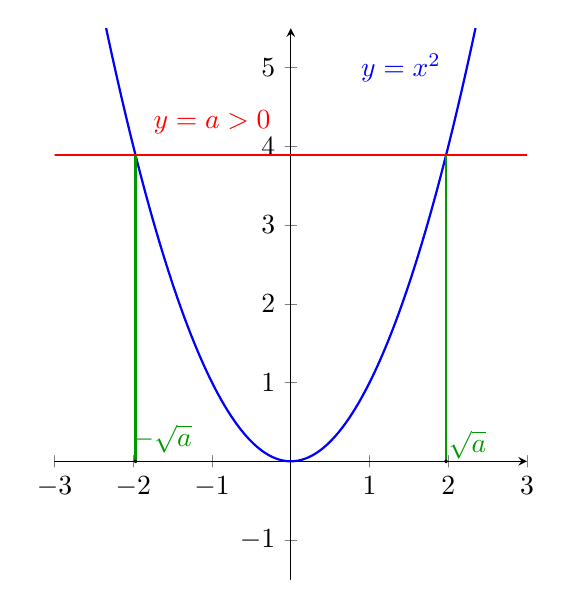
\begin{tikzpicture}[line cap=round,line join=round,>=triangle 45,x=1.0cm,y=1.0cm]
\begin{axis}[
x=1.0cm,y=1.0cm,
axis lines=middle,
xmin=-3.0,
xmax=3.0,
ymin=-1.5,
ymax=5.5,
xtick={-3.0,-2.0,...,3.0},
ytick={-1.0,0.0,...,5.0},
]
\clip(-3.,-1.5) rectangle (3.,5.5);
\draw[line width=0.8pt,color=qqqqff,smooth,samples=100,domain=-3.0:3.0] plot(\x,{(\x)^(2.0)});
\draw [line width=0.8pt,color=qqzzqq] (1.9718613223804418,3.8882370746999446)-- (1.9718613223804418,0.);
\draw [line width=0.8pt,color=qqzzqq] (-1.9718613223804418,3.8882370746999446)-- (-1.9718613223804418,0.);
\draw [line width=0.8pt,color=ffqqqq,domain=-3.:3.] plot(\x,{(-15.334128599692987-0.*\x)/-3.9437226447608835});
\begin{scriptsize}
                                
\draw [color=ffqqqq] (-1.,4.3) node {$y = a > 0 $};
\draw [color=qqqqff] (1.4,5) node {$y = x^{2} $};
\draw [fill=qqzzqq] (-1.9718613223804418,0.) circle (0.5pt);
\draw[color=qqzzqq] (-1.6325269105708164,0.2810659686932928) node {$- \sqrt a$};
\draw [fill=qqzzqq] (1.9718613223804418,0.) circle (0.5pt);
\draw[color=qqzzqq] (2.242795179422387,0.20524444954125187) node {$\sqrt a$};
\end{scriptsize}
\end{axis}
\end{tikzpicture}
\end{center}

$f (x) = x^{2}$ est injective sur $\mathbb{R}_{+}$ ou sur $\mathbb{R}_{-}$ mais
non injective sur $\mathbb{R}$ 

\item Repère de l'exemple sur la surjection $$f(x) = \frac{x^{2}}{x+1},
\quad x \neq -1$$
Soit $a, b \in \mathbb{R} \tq f(a) = f(b)$

\[
\begin{split}
\frac{a^{2}}{a+1}= \frac{b^{2}}{b+1} &\iff a^{2}
\cdot (b+1) = b^{2} \cdot (a+1)\\
&\iff a^{2}b + a^{2} - b^{2}a  - b^{2} = 0\\
&\iff ab \cdot (a-b) + (a+b)\cdot(a-b) = 0\\
&\iff (a-b) \cdot [a \cdot b + (a+b)] = 0
\end{split}
\]

$a \cdot b + a + b = 0$  est un "générateur de
contre-exemples".

En effet tout $(a, b) \in \mathbb{R}^{2}$ vérifiant cette
relation est un contre-exemple à l'injectivité de $f$. $$a =
3, \quad \quad \quad b = - \frac{3}{4}$$

Sont tels que $a \neq b$ et $f(a) = f(b)$.

$f$ est non injective.
                
\item Bijection et fonction réciproque

\paragraph{Définition:}
                
$f$ est bijective si elle est injective \textbf{et} surjective

En d'autres termes $f : A \to B$ est bijective si tout $y \in
B$  admet un unique antécédent.

\paragraph{Définition:}
                
$f: A \to B$ bijective si il existe une unique fonction, notée
$f^{-1}$, appelée fonction réciproque de $f$ 

Vérifiant:

$$f^{-1} \circ f = id_{A} \quad \quad \quad \text{ et } \quad
\quad \quad f \circ f^{-1} = id_{B}$$

\[
\begin{split}
f^{-1} : B &\to A\\
x &\mapsto y = f^{-1}(x)
\end{split}
\]
avec
$$x = f(y)$$

\paragraph{Exemple:}
                
\[
\begin{split}
f : \mathbb{R} &\to \mathbb{}\\
x &\mapsto y = x - x^{2}
\end{split}
\]

Restreindre les ensembles de départ et d'arrivée de sorte que
$f$ devienne bijective.

Puis déterminer $f^{-1}$ 

\begin{itemize}
\item Surjection

On cherche $$Im_{f} = \left\{y \in \mathbb{R}\ |\
\exists x \in \mathbb{R}, y = f(x)\right\}$$

\[
\begin{split}
&y = x - x^{2} \iff x^{2} - x + y = 0 \\
&\Delta = (-1)^{2} - 4 \cdot y = 1 - 4y \\
&\Delta \geq 0 \iff y \leq \frac{1}{4} \\
& Im_{f} = ] -\infty; \frac{1}{4}]\\
\end{split}
\]

\item Injection
Soit $a, b \in \mathbb{R}, \tq f(a) = f(b)$ 

\[
\begin{split}
&a - a^{2}= b - b^{2}\\
\iff & a^{2} - b ^{2} - a + b = 0\\
\iff & (a - b) (a+b) - (a-b) = 0\\
\iff & (a - b) \cdot [(a+b) - 1] = 0\\
\end{split}
\]

Comment restreindre l'ensemble de départ et
d'arrivée pour rendre $f$ injective, sans modifier
$Im_{f}$?

Il faut rendre le générateur de contre-exemple
"inopérant".

$$a + b = 1 \implies a - \frac{1}{2} = \frac{1}{2}
- b$$

$$A =\ \left]- \infty; \frac{1}{2}\ \right] \text{
ou } A  = \left[\ \frac{1}{2}; + \infty\ \right[$$

Alors 
$$ f: \left[\ \frac{1}{2}; + \infty\ \right[ \to
\left] - \infty; \frac{1}{4} \right] $$
est bijective.
\end{itemize}

Pour déterminer $f^{-1}$ , ou résoudre 
$$y = f(x)$$
par rapport à $x$ en prenant $y$ comme paramètre
$$y = x - x^{2} \iff x^{2} - x + y = 0$$
\[
\begin{split}
\Delta &= 1 - 4y\\
x &= \frac{1 \pm \sqrt{1 - 4y}}{2}, \quad \quad \left(y \in
\left] - \infty; \frac{1}{4} \right]\right)
\end{split}
\]

Or
$$x \in \left[ \frac{1}{2}; + \infty \right[$$
donc
$$ x = \frac{1 + \sqrt{1 - 4y}}{2}$$

\[
\begin{split}
f^{-1}: \left] - \infty; \frac{1}{4} \right] &\to
\left[ \frac{1}{2}; + \infty \right[\\
x &\mapsto \frac{1+ \sqrt{1 - 4y}}{2}
\end{split}
\]

\[
\begin{split}
id_{A}: A &\to A,\\
x &\mapsto A\\
id_{B}: B &\to B,\\
x &\mapsto x\\
\end{split}
\]
\end{enumerate}
\end{enumerate}


\section{Limite d'une fonction}
\label{sec:limite_d_une_fonction}

\subsection{Limite à infini}
\label{sub:limite_a_infini}

\paragraph{Définitions:}

\begin{enumerate}
\item $ \lim\limits_{x \to + \infty} f (x) = a, (a \in \mathbb{R})$  si
$$\forall \epsilon > 0, \exists M \in \mathbb{R} (M = M(\epsilon)) \tq
x \geq M (x \in D_{\text{déf}}) \implies |f(x) - a| < \epsilon$$

\begin{center}
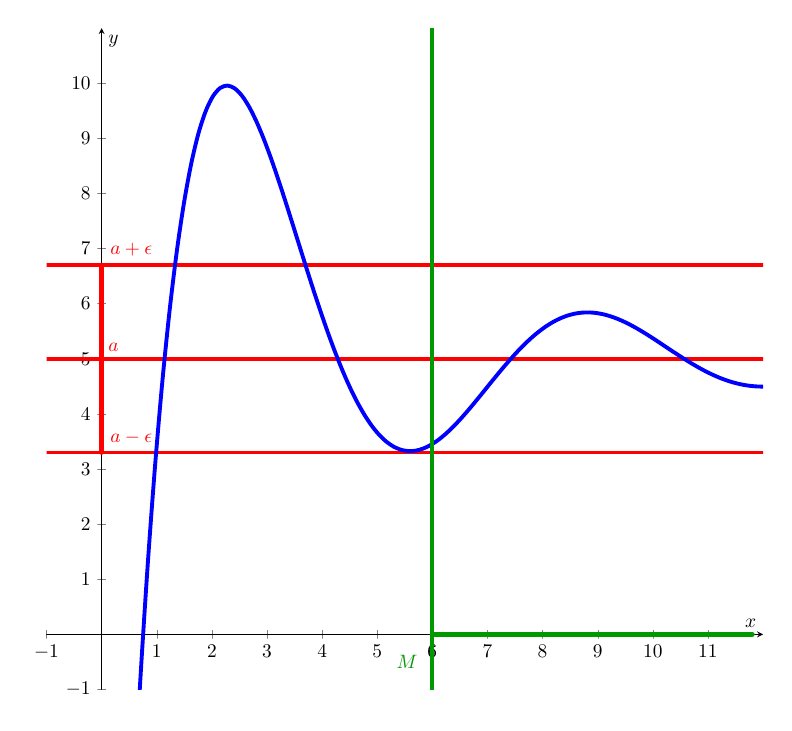
\begin{tikzpicture}[line cap=round,line join=round,>=triangle 45,x=1.0cm,y=1.0cm,
scale=.7]
\begin{axis}[
x=1.0cm,y=1.0cm,
axis lines=middle,
xmin=-1.0,
xmax=12.0,
ymin=-1.0,
ymax=11.0,
xtick={-1.0,0.0,...,11.0},
ytick={-1.0,0.0,...,10.0},
ylabel={$y$}, 
xlabel={$x$}, 
]
\clip(-1.,-1.) rectangle (12.,11.);
\draw[line width=4.pt] (-1.784804465134557,12.320336209179601) -- (1.762247575333074,12.320336209179601);
\draw [line width=2.pt,color=ffqqqq,domain=-1.:12.] plot(\x,{(--5.-0.*\x)/1.});
\draw [line width=2.pt,color=ffqqqq,domain=-1.:12.] plot(\x,{(--6.7-0.*\x)/1.});
\draw [line width=2.pt,color=ffqqqq,domain=-1.:12.] plot(\x,{(--3.3-0.*\x)/1.});
\draw[line width=2.pt,color=qqqqff,smooth,samples=100,domain=-1.0:12.0] plot(\x,{(-100.0*sin(((\x)+2.0)*180/pi))/((\x)+2.0)^(2.0)+5.0});
\draw [line width=2.pt,color=qqzzqq] (6.,-1.) -- (6.,11.);
\draw [line width=2.4pt,color=ffqqqq] (0.,6.7) node [anchor=south west] {$a + \epsilon$}-- (0.,3.3)
node [anchor=south west] {$a - \epsilon$};
\draw [line width=2.8pt,color=qqzzqq,domain=6.0:11.8] plot(\x,{(-0.-0.*\x)/2.10663383862404});
\begin{scriptsize}
\draw [fill=black] (-0.6142772917802388,12.320336209179601) circle (2.5pt);
\draw[color=ffqqqq] (0,5) node [anchor=south west] {$a$};
\draw[color=qqzzqq] (5.5398579984311,-0.49338928700971646) node {$M$};
\end{scriptsize}
\end{axis}
\end{tikzpicture}
\end{center}

\item $ \lim\limits_{x \to \infty} f (x) = a$  si
$$\forall \epsilon > 0, \exists N \in \mathbb{R} (N = N (\epsilon))
\tq x < N (x \in D_{\text{déf}}) \implies |f (x) - a| < \epsilon $$
\end{enumerate}

\paragraph{Exemple:}

Montrons que $$ \lim_{x \to - \infty} \frac{1}{x^{2}} = 0$$

Soit $\epsilon > 0$  donné

Montrons qu'il existe $N \in \mathbb{R}$  tel que

\[
\begin{split}
x < N &\implies | \frac{1}{x^{2}} - 0 | < \epsilon\\
&\iff |\frac{1}{x^{2}}| < \epsilon\\
&\iff \frac{1}{x^{2}} < \epsilon\\
&\iff |x| > \frac{1}{\epsilon}\\
&\iff x \in \left] - \infty; - \frac{1}{\sqrt{\epsilon}}\ \right[ \cup \left] \frac{1}{\sqrt{\epsilon}}; + \infty \right[
\end{split}
\]

Donc tout $N \leq - \frac{1}{\sqrt{\epsilon}}$ convient, car $$x < N ( \text{
avec }  N \leq - \frac{1}{\sqrt{\epsilon}}) \implies |\frac{1}{x^{2}} - 0| <
\epsilon$$

\cqfd

\paragraph{Théorème de caractérisation par les suites:}

$f$  admet une limite $x \to \infty$ et $$ \lim_{x \to \infty} f(x) = a$$

si et seulement si pour toute la suite  $x_{n}$ qui diverge vers $\infty$, on
a $$ \lim_{x \to \infty} f(x_{n}) = a$$

\paragraph{Exemple:}

Montrons que $\lim\limits_{x \to \infty} \sin(x)$ n'existe pas.

\begin{itemize}
\item Soit $x_{n} = n \cdot \pi, \quad n \in \mathbb{N}^{*}$ 
$$ \lim_{n \to \infty} x_{n} = + \infty$$ et $$ \lim_{n \to \infty}
\sin(x_{n}) = \lim_{n \to \infty} \sin(n \cdot \pi) = 0$$
\item Soit $y_{n} =  \frac{\pi}{2} + n \cdot 2 \pi, \quad n \in \mathbb{N}^{*}$ 
$$ \lim_{n \to \infty} y_{n} = + \infty$$ et $$ \lim_{n \to \infty}
\sin(y_{n}) = \lim_{n \to \infty} \sin(n \cdot \frac{\pi}{2}) = 1$$
\end{itemize}

Donc $\lim\limits_{x \to + \infty} \sin(x)$  n'existe pas.


\paragraph{Définitions:}

Limites impropre

\begin{enumerate}
\item $\lim\limits_{x \to + \infty} f (x) = + \infty$ si $$\forall A >
0,\quad \exists M \in \mathbb{R} \tq x > M \implies f(x) > A$$

\item $\lim\limits_{x \to + \infty} f (x) = - \infty$ si $$\forall B <
0,\quad \exists M \in \mathbb{R} \tq x > M \implies f(x) < B$$

\item $\lim\limits_{x \to - \infty} f (x) = + \infty$ si $$\forall A >
0,\quad \exists N \in \mathbb{R} \tq x < N \implies f(x) > A$$

\item $\lim\limits_{x \to - \infty} f (x) = - \infty$ si $$\forall B <
0,\quad \exists N \in \mathbb{R} \tq x < N \implies f(x) < B$$
\end{enumerate}

\paragraph{Exemple:}

$$ \lim_{x \to - \infty} x^{2} = + \infty$$

Soit $A > 0, \quad \exists? N \in \mathbb{R} \tq x < N \implies$ 

\[
\begin{split}
\implies & x^{2} > A \iff |x| = \sqrt{A}\\
\implies & x \in \left] - \infty; - \sqrt{A} \right] \cup
\left]\sqrt{A}; + \infty \right[
\end{split}
\]

Donc tout $x < N$ convient. \cqfd

\paragraph{Opération sur les limites}

\begin{enumerate}
\item Si $\lim\limits_{x \to \infty} f (x) = a  \text{ et } \lim\limits_{x
\to \infty} g (x) = b $ alors

$$ \lim_{x \to \infty} |f(x)| = |a|, \quad \lim_{x \to \infty}
\left(f(x) \pm g(x)\right) = a \pm b$$

$$ \lim_{x \to \infty} \left( f (x) \cdot g(x)\right) = a \cdot b, \quad 
\lim_{x \to  \infty} \left( \frac{f(x)}{g(x)}\right) = \frac{a}{b},
\quad ( \text{ si }  b \neq 0) $$

\item Si $\lim\limits_{x \to \infty} f (x) = a  \text{ et } \lim\limits_{x
\to \infty} g (x) = + \infty $ alors

$$\lim_{x \to \infty} \left(f(x) + g(x)\right) = + \infty$$
$$\lim_{x \to \infty} \left( \frac{f(x)}{g(x)}\right) = 0$$

\item Si $\lim\limits_{x \to \infty} f (x) = + \infty  \text{ et } \lim\limits_{x \to \infty} g (x) = + \infty $ alors

$$\lim_{x \to \infty} \left(f(x) + g(x)\right) = + \infty$$
$$\lim_{x \to \infty} \left(f(x) \cdot g(x)\right) = + \infty$$
\end{enumerate}

\paragraph{Cas d'indétermination}
\label{par:cas_d_indetermination}

Si $$\lim\limits_{x \to \infty} f (x) = 0, \lim\limits_{x \to \infty} g (x) = 0  \text{ et } 
\lim\limits_{x \to \infty} i (x) = + \infty, \lim\limits_{x \to \infty} h (x) = + \infty $$ alors
on ne peut rien dire à priori des limites suivante 
$$ \lim_{x \to \infty} (h(x) - i(x)) = "\infty - \infty"$$
$$ \lim_{x \to \infty} \left(\frac{f(x)}{g(x)}\right) = "\frac{0}{0}"$$

$$ \lim_{x \to \infty} \left(\frac{h(x)}{i(x)}\right) = "\frac{\infty}{\infty}"$$





\paragraph{Quelque théorème importants}


\begin{enumerate}
\item \textbf{Théorème des 2 gendarmes} 

Soient $d (x), g (x)$  toutes les fonctions telles que $$\exists M > 0
\text{ avec } g (x) \leq x \leq d (x), \quad \forall x > M$$
Alors si $$ \lim_{x \to + \infty} g (x) = \lim_{x \to + \infty} d (x) = a$$
on a $$\lim_{x \to + \infty} f (x) = a$$

Énoncé analogue pour $x \to - \infty$ 

\paragraph{Corollaire des 2 gendarmes}
\label{par:corollaire_des_2_gendarmes}
        
$$ \lim_{x \to + \infty} | f (x) | = 0 \implies \lim_{x \to + \infty} f (x)
= 0$$
$$ [ \underbrace{|f(x)|}_{\to 0} \leq f (x) \leq \underbrace{ | f (x) |}_{\to 0} \quad \Box]$$
\item \textbf{Théorème du gendarme}(ou du chien méchant)
Soient $f (x), g (x)$  toutes les fonctions telles que $$\exists M > 0
\text{ avec } f (x) \geq g (x), \quad \forall x > M$$
Alors si $$ \lim_{x \to + \infty} g (x)  = + \infty$$ on a $$ \lim_{x \to + \infty} f
(x) = + \infty$$

Énoncé analogue pour $x \to - \infty,  y \to - \infty$ 

\item \textbf{Théorème "}$0\ \cdot$ borné\textbf{"}

Soient $f, g$ deux fonctions telles que $\lim\limits_{x \to + \infty}
f (x) = 0$  et $\exists M > 0$ avec $g(x)$ est borné sur $[M; + \infty[$ 

Alors $$ \lim_{x \to + \infty} f(x) \cdot g(x) = 0$$

[Par hypothèse $$ \exists A > 0 \tq |g(x)| \leq A, \quad x > M $$ $$0
\leq |f(x) \cdot g(x)| = |f(x)|\cdot|g(x)| \leq
\underbrace{|f(x)|}_{\to 0} \cdot A$$ Donc d'après les deux
gendarmes: $|f(x) \cdot g(x) |\xrightarrow[x \to \infty]{} 0$ d'après
son corolaire: $f(x) \cdot g(x) \xrightarrow[x \to + \infty]{} 0$ ]

Énoncé analogue pour $x \to - \infty$ 

\paragraph{Exemple:}
        
$f(x) = \frac{\sin(x)}{x},  \quad x \to + \infty$ 

$$ \lim_{x \to \infty} f(x) = \lim_{x \to \infty} \underbrace{\frac{1}{x}}_{\to 0} \cdot
\underbrace{\sin(x)}_{\text{borné}} = 0$$

Or $f$ est paire, donc $\lim\limits_{x \to - \infty} f(x) = 0$ 

\item \textbf{Théorème "}$\infty \cdot \text{ signe constant}$ \textbf{"} 

\begin{itemize}
\item Si $\lim\limits_{x \to + \infty} f(x) = + \infty$ et $g (x)
\geq m > 0$ sur un voisinage de $+ \infty$ .


Alors $$ \lim_{x \to + \infty} f(x) \cdot g(x) = + \infty$$

\item Si $\lim\limits_{x \to + \infty} f(x) = + \infty$ et $g (x)
\leq m < 0$ sur un voisinage de $+ \infty$ .


Alors $$ \lim_{x \to + \infty} f(x) \cdot g(x) = - \infty$$
\end{itemize}

Énoncé analogue pour $x \to - \infty,  y \to - \infty$ 

\item \textbf{Théorème "}$\infty\ +$ borné\textbf{"} 
Si $\lim\limits_{x \to + \infty} f(x) = + \infty$ et $g (x)$ est borné
sur un voisinage de $+ \infty$. Alors $$ \lim_{x \to + \infty} (f(x) +
g(x)) = + \infty$$

Énoncé analogue pour $x \to - \infty,  y \to - \infty$ 
\end{enumerate}


\paragraph{Exemples:}

\begin{enumerate}
\item $\lim\limits_{x \to - \infty} (x + \sin(x)) = - \infty$ 

\item $f (x) = \frac{x \cdot \sin(x)}{( \cos(x) - 2) \cdot (x + \sqrt{x^{4}+x^{2}})},
\quad x \to - \infty$ 

\[
\begin{split}
& \frac{x \cdot \sin(x)}{( \cos(x) - 2) \cdot (x + \underbrace{|x|}_{=
- x} \cdot \sqrt{ x^{2} +1})}, \quad x < 0\\
& \frac{ \overbrace{\sin(x)}^{\text{borné}}}{\underbrace{(\cos(x) - 2)}_{\leq
-1 < 0} \cdot \underbrace{(-1 \cdot \sqrt{ x^{2} +1})}_{\to -
\infty}} \xrightarrow[x \to - \infty]{} 0 \quad \quad \text{("$0 \cdot$ borné")}\\
\end{split}
\]
\end{enumerate}


\subsection{Valeurs limite en $x_{0}$ }
\label{sub:valeurs_limite_en_x__0_}


\paragraph{Définition:}

Soit $x_{0} \in \mathbb{R}$. On appelle voisinage pointé de $x_{0}$, tout
voisinage de $x_{0}$, privé de $x_{0}$

\paragraph{Exemple:}

L'ensemble
$$\{ x \in \mathbb{R} | 0 < |x - x_{0}| < \delta \}$$
est appelé $\delta$-voisinage pointé de $x_{0}$.

En effet: $0 < |x - x_{0}| < \delta$ 

$$\iff x \in ]x_{0} - \delta; x_{0}[ \cup ]x_{0}; x_{0} + \delta[$$

\paragraph{Définition:}

Soient $x_{0} \in \mathbb{R}$ et $f$ une fonction définie sur un voisinage
pointé de $x_{0}$. $$ \lim_{\stackbin[(x \neq x_{0})]{}{x \to x_{0}}} f(x) = a, \text{ si } \forall \epsilon
> 0, \exists \delta > 0\ (\delta = \delta(\epsilon))$$ tels que $$0 < |x -
x_{0}| < \delta \implies |f(x) - a| < \epsilon$$

$ \lim_{x \to x_{0}} f(x) = a $ si et seulement si tout $\epsilon$-voisinage de $a$ contient
l'image par $f$ d'un $\epsilon$-voisinage pointé de $x_{0}$ 

\begin{enumerate}
\item \textbf{Théorème de caractérisation par les suites} 

$\lim\limits_{x \to x_{0}} f(x) = a$ si et seulement si pour toutes
suites $(r_{n})_{n \in \mathbb{N}^{*}}$ qui converge vers $x_{0}:
\lim\limits_{n \to \infty} x_{n} = x_{0}, \quad (x_{n} \neq x_{0})$ 

On a $$ \lim_{n \to \infty} f(x_{n}) = a$$

\paragraph{Exemple:}
        
$$f(x) = \left\{\begin{array}{lr}x, & \text{ si } x \leq 1\\ x^{2} +
1, & \text{ si } x>1\end{array}\right.$$
        
Montrons que $\lim\limits_{x \to 1} f (x)$ n'existe pas

\begin{itemize}
\item Soit $x_{n} = 1 - \frac{1}{n}$  $$x_{n} \to 1$$ et $$f(x_{n})
= 1 - \frac{1}{n} \xrightarrow[n \to \infty]{} 1$$

\item Soit $y_{n} = 1 + \frac{1}{n} (y_{n} > 1)$ $$ \lim_{n \to \infty} y_{n}
= 1$$
mais 

\[
\begin{split}
f (y_{n}) &= y_{n}^{2} + 1 \\
&= \left(1 + \frac{1}{n}\right)^{2} + 1\\
&= 2 + \frac{2}{n} + \frac{1}{n^{2}}\\
\end{split}
\]

$$ \lim_{n \to \infty} f(y_{n}) = 2 $$
\end{itemize}

Donc $\lim\limits_{f(x)}$ n'existe pas

\paragraph{Définitions:}
        
Limite à gauche et à droite de $x_{0}$ 

\begin{itemize}
\item $\lim\limits_{n \to x_{0}^{-}} f (x) = a $ Si 
$$\forall \epsilon > 0, \exists \delta > 0 (\delta = \delta(\epsilon))
\tq x_{0}-\delta < x < x_{0} \implies |f(x) - a| < \epsilon$$

\item $\lim\limits_{n \to x_{0}^{+}} f (x) = a $ Si 
$$\forall \epsilon > 0, \exists \delta > 0 (\delta = \delta(\epsilon))
\tq x_{0} < x < x_{0} + \delta \implies |f(x) - a| < \epsilon$$
\end{itemize}

Reprise de l'exemple précédent:
$$ \lim_{x \to x_{0}^{-}} f(x) = 1, \quad \lim_{x \to x_{0}^{+}} f(x)
= 2$$

\paragraph{Théorème}

$\lim\limits_{x \to x_{0}} f(x)$ existe si et seulement si 
$$ \lim_{x \to x_{0}^{-}} f(x) = \lim_{x \to x_{0}^{+}} f(x)$$
\end{enumerate}

\paragraph{Définition:}

Limites  infinies en $x_{0}$ 

\begin{itemize}
\item $\lim\limits_{x \to x_{0}} f(x) = + \infty$
$$\forall A > 0, \exists \delta > 0 (\delta = \delta(A)) \tq 0 < |x -
x_{0} | < \delta \implies f(x) > A$$
\item $\lim\limits_{x \to x_{0}} f(x) = - \infty$
$$\forall B < 0, \exists \delta > 0 (\delta = \delta(A)) \tq 0 < |x -
x_{0} | < \delta \implies f(x) < B$$
\end{itemize}


\paragraph{Exemple:}

Montrer que $$ \lim_{x \to 0} \frac{1}{x^{2}} = + \infty$$
Soit $A > 0$ donné, montrons que 
$$ \exists \delta > 0 \tq 0 < | x - 0| < \delta \implies \frac{1}{x^{2}} > A\\ $$
$$ \frac{1}{x^{2}} > A \iff x^{2} < \frac{1}{A} \iff |x| < \frac{1}{\sqrt{A}}
\iff | x - 0 | < \frac{1}{\sqrt{A}} $$
Donc tout $\delta \leq \frac{1}{\sqrt{A}}$ convient, car $$0 < | x - 0| <
\delta, (\text{ avec } \delta \leq \frac{1}{\sqrt{A}}) \implies \frac{1}{x^{2}}
> A$$

\paragraph{Définitions:}

Limites infinies à gauche et à droite en $x_{0}$

\begin{itemize}
\item $\lim\limits_{x \to x_{0}^{+}} f(x) = + \infty$ si
$$\forall A > 0, \exists \delta > 0 \quad \tq \quad x_{0} < x < x_{0} + \delta
\implies f(x) > A$$

\item $\lim\limits_{x \to x_{0}^{-}} f(x) = + \infty$ si
$$\forall A > 0, \exists \delta > 0 \quad \tq \quad x_{0} - \delta < x < x_{0}
\implies f(x) > A$$

\item $\lim\limits_{x \to x_{0}^{+}} f(x) = - \infty$ si
$$\forall B < 0, \exists \delta > 0 \quad \tq \quad x_{0} < x < x_{0} + \delta
\implies f(x) < B$$

\item $\lim\limits_{x \to x_{0}^{-}} f(x) = + \infty$ si
$$\forall B < 0, \exists \delta > 0 \quad \tq \quad x_{0} - \delta < x < x_{0}
\implies f(x) < B$$
\end{itemize}

\paragraph{Exemple:}

Montrons que $\lim\limits_{x \to 0^{-}} \frac{1}{x} = - \infty$

Soit $B > 0$ donné, montrons que $$\exists \delta > 0 \tq 0 - \delta < x < 0
\implies \frac{1}{x} < B \implies \frac{1}{x} < B \iff x > \frac{1}{B}, \quad (x, B
< 0)$$
Donc tout $\delta > 0$ vérifiant $$\frac{1}{B} < - \delta < 0$$ convient $(\delta
< - \frac{1}{B})$ car $$0 - \delta < x < 0 \quad (\text{avec } - \delta > \frac{1}{B})
\implies \frac{1}{x} > B$$

\cqfd

\paragraph{Remarque:}

Tout les théorèmes et règles de calcul concernant les limites lorsque $x \to
\pm \infty$ restent valables lorsque $x \to x_{0}$

\paragraph{Exemple:}

$$ \lim_{x \to 1} \frac{x - \sqrt{ 2 - x }}{\sqrt[3]{1 - x^{2}}} \cdot \cos \left(\frac{1}{1-x}\right) $$

\begin{center}
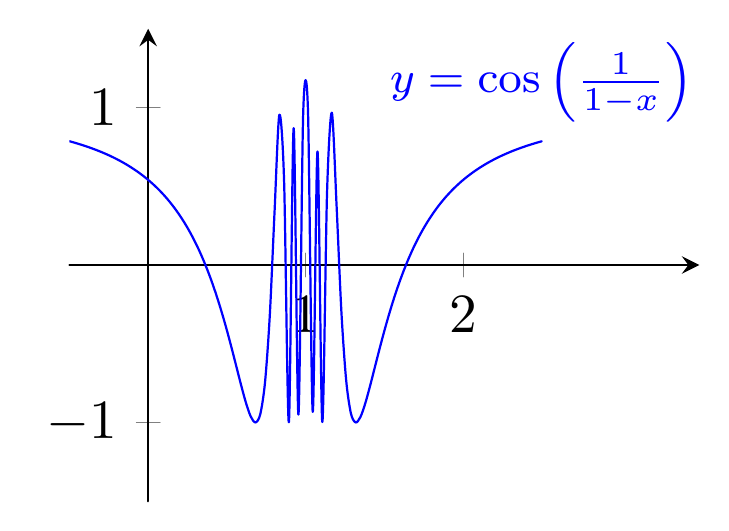
\begin{tikzpicture}[line cap=round,line join=round,>=triangle 45,x=1.0cm,y=1.0cm,scale=2]
\begin{axis}[
x=1.0cm,y=1.0cm,
axis lines=middle,
xmin=-0.5,
xmax=3.5,
ymin=-1.5,
ymax=1.5,
xtick={-0.0,1.0,...,2.0},
ytick={-1.0,0.0,...,1.0},]
\draw[line width=0.4pt,color=qqqqff,smooth,samples=100,domain=-0.5:2.5] plot(\x,{cos((1.0/(1.0-(\x)))*180/pi)})
node [font=\footnotesize, anchor = south] {$y = \cos\left(\frac{1}{1-x}\right)$};
\end{axis}
\end{tikzpicture}
\end{center}

\[
\begin{split}
\lim_{x \to  1}& \frac{x - \sqrt{2-x}}{\sqrt[4]{1 - x^{2}}} = 0\\
\lim_{x \to  1}& \frac{x - \sqrt{2-x}}{\sqrt[4]{1 - x^{2}}} : \text{ FI } \quad "\frac{0}{0}"\\
\lim_{x \to  1}& \frac{x^{2} - (2 - x )}{\sqrt[3]{(1-x^{2})}
\cdot (x + \sqrt{2 - x })} = \\
\lim_{x \to  1}&  \frac{(x - 1) \cdot (x + 2)}{\sqrt[3]{(1-x)\cdot(1+x)}
\cdot (x + \sqrt{2 - x })} = \\
\lim_{x \to  1}& \frac{\sqrt[3]{(x-1)^{2}} \cdot (x+2)}{\sqrt[3]{- 1 - x }
\cdot (x + \sqrt{2 - x })} = 0 \\
\end{split}
\]

Donc $$ \lim_{x \to 1} \underbrace{ \frac{x - \sqrt{2 - x }}{\sqrt[3]{ 1 - x ^{2}}}}_{\to 0} \cdot
\underbrace{\cos \left(\frac{1}{1-x}\right)}_{\text{borné}} = 0$$


\subsection{Infiniment petits équivalents (IPE)}
\label{sub:infiniment_petits_equivalents_ipe_}

\paragraph{Définition:}

Soient $f$ et $g$ 2 fonctions définies sur un voisinage pointé de $x_{0}$.

$f$ et $g$ sont des IPE $( x \to x_{0})$ si et seulement si
\begin{itemize}
\item $ \lim\limits_{x \to x_{0}} f(x) = \lim_{x \to x_{0}} g(x) = 0 \quad (\text{IP})$
\item $ \lim\limits_{x \to x_{0}} \frac{f(x)}{g(x)} = 1 \quad (\text{E})$
\end{itemize}

On écrit alors $f \sim g \quad (x \to x_{0})$

Montrons que $$\sin(x) \sim x \quad x \to 0$$

\begin{center}
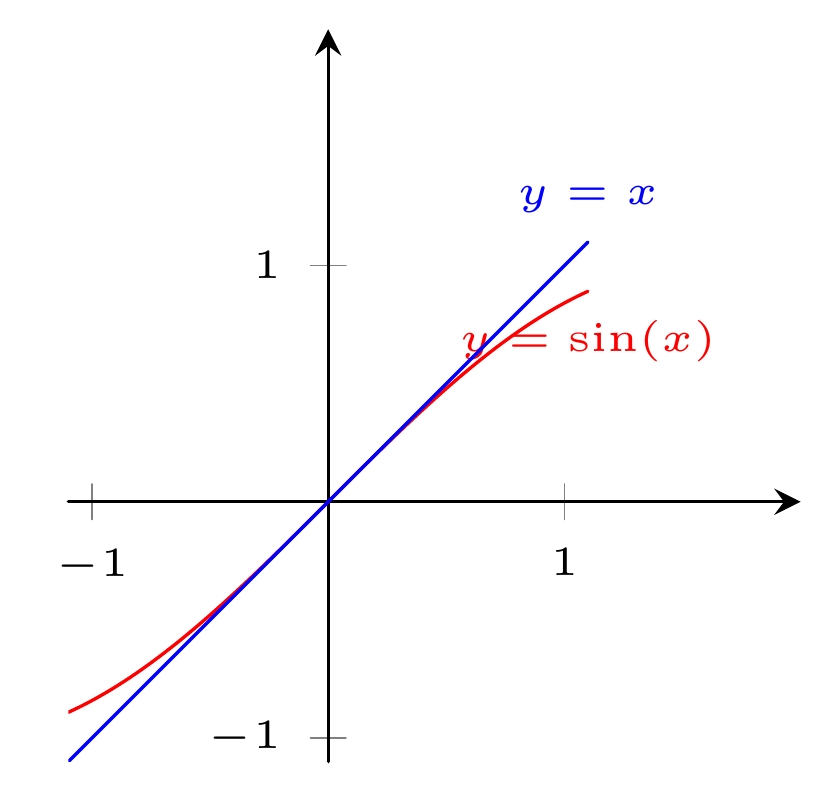
\begin{tikzpicture}[line cap=round,line join=round,>=triangle 45,x=1.0cm,y=1.0cm,
scale=3]
\begin{axis}[
x=1.0cm,y=1.0cm,
axis lines=middle,
xmin=-1.1,
xmax=2,
ymin=-1.1,
ymax=2,
xtick={-1.0,0.0,...,1.0},
ytick={-1.0,0.0,...,1.0},
tick label style = {font=\tiny} ]
\draw[line width=0.4pt,color=ffqqqq,smooth,samples=100,domain=-1.1:1.1] plot(\x,{sin(((\x))*180/pi)})node [anchor=north, font=\tiny] {$y = \sin(x)$};
\draw[line width=0.4pt,color=qqqqff,smooth,samples=100,domain=-1.1:1.1] plot(\x,{(\x)})
node [anchor=south, font=\tiny] {$y = x$};
\begin{scriptsize}
\draw[color=ffqqqq] (-2.1231414942035336,-0.8751128172227396) node {$f$};
\draw[color=qqqqff] (-2.1231414942035336,-2.208249722038624) node {$g$};
\end{scriptsize}
\end{axis}
\end{tikzpicture}
\end{center}

Soit $ 0 < x < \frac{\pi}{2}$

\begin{center}
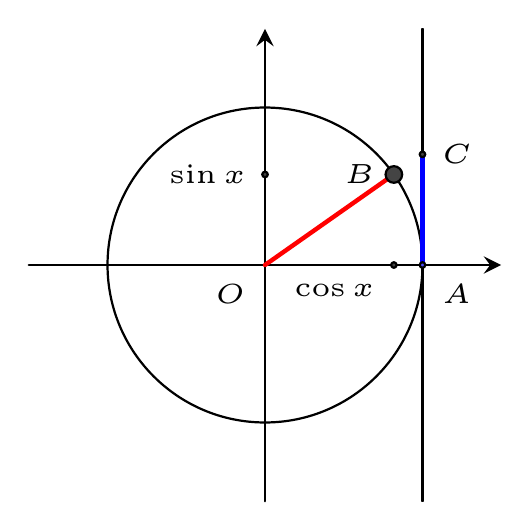
\begin{tikzpicture}[line cap=round,line join=round,>=triangle 45,x=1.0cm,y=1.0cm, scale = 2]
\begin{axis}[
x=1.0cm,y=1.0cm,
axis lines=middle,
xmin=-1.5,
xmax=1.5,
ymin=-1.5,
ymax=1.5,
xticklabels={},
yticklabels={}]
\clip(-1.5,-1.5) rectangle (1.5,1.5);
\draw [line width=0.4pt] (0.,0.) circle (1.cm) node [anchor = north
east, font=\tiny] {$O$};
\draw [line width=0.8pt,color=ffqqqq] (0.,0.)-- (0.8182771110644109,0.5748239465332684);
\draw [line width=0.4pt] (1.,-1.5) -- (1.,1.5);
\draw [line width=0.8pt,color=qqqqff] (1.,0.7024807840287017)-- (1.,0.);
\begin{scriptsize}
\draw [fill=ududff] (1.,0.) circle (0.5pt) node[font = \tiny, anchor = north west] {$A$};
\draw [fill=black] (-1.375668034475281,1.8965376227529331) circle (2pt);
\draw [fill=uuuuuu] (0.8182771110644109,0.5748239465332684) circle (1.5pt) node [anchor = east, font = \tiny] {$B$};
\draw [fill=uuuuuu] (0.8182771110644109,0.) circle (0.5pt) node[font = \tiny, anchor = north east] {$\cos x$};
\draw [fill=uuuuuu] (0.,0.5748239465332684) circle (0.5pt) node[font = \tiny, anchor = east] {$\sin x$};
\draw [fill=uuuuuu] (1.,0.7024807840287017) circle (0.5pt) node[font = \tiny, anchor = west] {$C$};
\end{scriptsize}
\end{axis}
\end{tikzpicture}
\end{center}


\[
\begin{split}
&\dim (\Delta AOB) < \dim (O\hat A B) < \dim (\Delta OAC)\\
\iff & \frac{1}{2} \cdot 1 \cdot \sin(x) < \frac{1}{2} \cdot x \cdot
1^{2} < \frac{1}{2} \cdot 1 \cdot \tan(x)\\
\iff & \sin(x) < x < \tan(x) \\
\iff & 1 < \frac{x}{\sin(x)} < \frac{1}{\cos(x)}\\
\iff & \underbrace{\cos(x)}_{\to 1} < \frac{\sin(x)}{x} < 1\\
\end{split}
\]

Théorème des 2 gendarmes: $$\lim_{x \to 0^{+}}  \frac{\sin(x)}{x} = 1$$
Or $\frac{\sin(x)}{x}$ est paire donc $$\lim_{x \to 0} \frac{\sin(x)}{x} = 1$$
De plus $$\lim_{x \to 0} \sin(x) = \lim_{x \to 0} x = 0$$
donc $$\sin(x) \sim x \quad  (x \to 0)$$


\paragraph{Propriété:}

Si $f_{1} \sim g_{1}$ et $f_{2} \sim g_{2}$ au voisinage de $x_{0}$, alors $$f_{1}
\cdot f_{2} \sim g_{1} \cdot g_{2} $$

\Warning Attention: En général
$$f_{1} \sim g_{1}  \text{ et } f_{2} \sim g_{2} \centernot\implies f_{1} + f_{2}
\sim g_{1} + g_{2} $$

Contre-exemple: 
$$ x \sim (x + x^{2}) \text{ et } x \sim (-x + x^{2}) \quad (x \to 0)$$
Or
$$\frac{x-x}{(x+x^{2})+(-x + x^{2})} = \frac{0}{2x^{2}} {\text{ \Large!}}$$

D'où la règles d'utilisation des IPE.

Dans un calcul de limit on peut remplacer une fonction par son IPE, uniquement
dans une \textbf{expression factorisée} et \textbf{\underline{jamais}} dans une somme.

\paragraph{Exemples:}

\begin{enumerate}
\item $\lim\limits_{x \to 0} (1 - \cos(x)) = 0$ et $$1 - \cos(x) = 2 \sin\left(\frac{x^{2}}{2}\right)
\sim 2 \cdot \left(\frac{x}{2}\right)^{2} = \frac{x^{2}}{2}$$
donc $$1 - \cos(x) \sim \frac{x^{2}}{2}, \quad (x \to 0)$$

\begin{center}
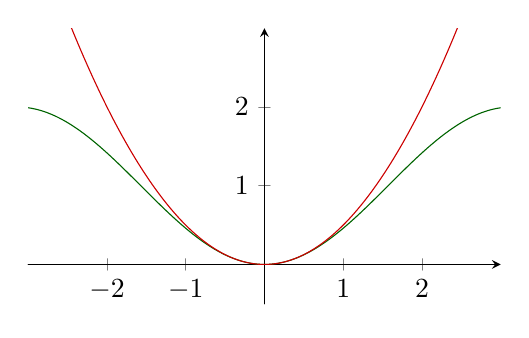
\begin{tikzpicture}[line cap=round,line join=round,>=triangle 45,x=1.0cm,y=1.0cm]
\begin{axis}[
x=1.0cm,y=1.0cm,
axis lines=middle,
xmin=-3.0,
xmax=3.0,
ymin=-0.5,
ymax=3.0,
xtick={-2.0,...,2.0},
ytick={-0.0,1.0,...,2.0},]
\clip(-3.,-0.5) rectangle (3.,3.);
\draw[line width=0.4pt,color=qqwuqq,smooth,samples=100,domain=-3.0:3.0] plot(\x,{1.0-cos(((\x))*180/pi)});
\draw[line width=0.4pt,color=ccqqqq,smooth,samples=100,domain=-3.0:3.0] plot(\x,{(\x)^(2.0)/2.0});
\end{axis}
\end{tikzpicture}
\end{center}

\item $\lim\limits_{x \to 0} \tan(x) = 0$ et $$ \lim_{x \to 0} \frac{\tan(x)}{x}$$
et $$\lim_{x \to 0} \frac{\tan(x)}{x} = \lim_{x \to 0}
\underbrace{\frac{\sin(x)}{x}}_{\to 1} \cdot
\underbrace{\frac{1}{\cos(x)}}_{\to 1} = 1$$

Donc $$\tan(x) \sim x \quad (x \to 0)$$
\end{enumerate}

\paragraph{Exemple servant d'avertissement:}
\label{par:exemple_servant_d_avertissement_}

$$\lim_{x \to 0} \frac{2 \cdot \sin(x) - \sin(2x)}{x^{3}}$$

\[
\begin{split}
\text{ Lorsque }  x \to 0 \quad &2 \cdot \sin(x) \sim 2x \\
\text{ et } \quad & \sin(2x) \sim 2x
\end{split}
\]

Mais
$$ \lim_{x \to 0} \frac{2 \cdot \sin(x) - \sin(2x)}{x^{3}} \neq
\lim_{\substack{x \to 0 \\ x \neq 0}} \frac{2x - 2x}{x^{3}} = \lim_{x \to 0}
\frac{0}{x^{2}} = 0$$

$$\lim_{x \to 0} \frac{2 \cdot \sin(x) - \sin(2x)}{x^{3}} = \lim_{x \to 0}
\frac{2 \cdot \sin(x)\cdot \cos(x)}{x^{3}} = \lim_{x \to 0} \frac{2 \cdot
\sin(x) \cdot (1 - \cos(x))}{x^{3}} = \lim_{x \to 0} \frac{2 \cdot x \cdot
\frac{x^{2}}{2}}{x^{3}} = 1$$

\section{Continuité}

\paragraph{Définition:}

Soit $f$ définie sur un voisinage de $x_{0}$. $f$ est continue en $x_{0}$ si $$\lim_{x \to x_{0}} f(x)
= f (x_{0})$$

Cette définition comporte 3 exigences:
\begin{enumerate}
\item $f (x_{0})$ existe $(x_{0} \in \mathbb{D}_{\text{déf}})$
\item $\lim\limits_{x \to x_{0}} f (x)$ existe (vaut $a \in \mathbb{R}$)
\item $a = f (x_{0})$
\end{enumerate}

\paragraph{Définition analytique}
\label{par:definition_analytique}

$f$ est continue en $x_{0}$ si $$\forall \epsilon > 0, \exists \delta > 0 \tq
(x - x_{0}) < \delta \implies |f (x) - f (x_{0})| < \epsilon$$


\paragraph{Définition:}

$f$ est continue sur un ensemble $I = ]\ a, b\ [$ si $f$ est continue en tout
$x_{0} \in I$ et on écrit $f \in \mathbb{C}^{0}_{I}$ (la $O^e$ dérivé de $f$
continue sur l'intervalle $I$)


\paragraph{Exemples:}

\begin{enumerate}
\item Montrons que $\sin(x) \in \mathbb{C}^{0}_{\mathbb{R}}$

Soit $\epsilon > 0$ donné
\[
\begin{split}
&| \sin(x) - \sin(x_{0}) | = | 2 \cdot \cos\left(\frac{x+x_{0}}{2}\right)
\cdot \sin\left(\frac{x - x_{0}}{2}\right) | \leq \\
\leq & |2 \cdot \sin\left(\frac{x - x_{0}}{2}\right)| \leq |2
\cdot \frac{x - x_{0}}{2}| = |x-x_{0}|
\end{split}
\]
Donc tout $\delta \leq \epsilon$ convient car $$| x - x_{0} | < \delta
\quad (\text{avec } \delta \leq \epsilon) \implies | \sin(x) - \sin(x_{0})
| < \epsilon$$
\cqfd

Corollaire $\cos(x) \in \mathbb{C}^{0}_{\mathbb{R}}$ car $\cos(x) = \sin\left(\frac{\pi}{2} -
x\right)$

\item Montrer que $\sqrt{x}$ est contenue sur $\mathbb{R}^{*}_{+}$ 

Montrons que $\lim\limits_{x \to x_{0}} \sqrt{x} = \sqrt{x_{0}}$
$$ | \sqrt{x} - \sqrt{x_{0}}| = | \frac{x - x_{0}}{\sqrt{x} + \sqrt{x_{0}}}
| \leq | \frac{x - x_{0}}{\sqrt{x_{0}}}  = \frac{| x - x_{0}|}{\sqrt{x_{0}}}$$
Or $$\frac{| x - x_{0} |}{\sqrt{x_{0}}} < \epsilon \iff | x - x_{0} |
< \epsilon \sqrt{x_{0}}$$
Donc tout $$\delta \leq \epsilon \cdot \sqrt{x_{0}}$$ convient car $$|
x - x_{0} | < \delta \quad (\delta \leq \epsilon \cdot \sqrt{x_{0}})
\implies |\sqrt{x} - \sqrt{x_{0}}| < \epsilon$$
\end{enumerate}

\paragraph{Propriétés:}
Soit $f$ , $g$ continues en $x_{0}$ alors

\begin{itemize}
\item $|f|$ est continue en $x_{0}$
\item $f\pm g$ sont continue en $x_{0}$
\item $f \cdot g$ est continue en $x_{0}$
\item si $g(x_{0}) \neq 0, \frac{f}{g}$ est continue en $x_{0}$
\end{itemize}
Ces propriété sont la conséquence des propriétés sur la limite en $x_{0}$

\paragraph{Théorème:}

Soit $f$ et $g$ deux fonctions. $f$ définie sur un voisinage pointé de $x_{0}$.
Si $\lim\limits_{x \to x_{0}} = a$ et si $g$ est continue en $a$, alors $$\lim_{x \to x_{0}}
g (f (x)) = g ( \lim_{x \to x_{0}} f (x)) = g(a)$$

\paragraph{Corollaire:}

Soient $f$ continue en $x_{0}$ et $g$ continue en $f(x_{0})$. Alors $g \circ f$
est continue sur en $x_{0}$

[
\[
\begin{split}
\lim_{x \to x_{0}} g \circ f (x) &= \lim_{x \to x_{0}} g(f(x))\\
&= g \left( \lim_{x \to x_{0}} f(x)\right) \text{ car $g$ est
continue }\\
&= g(f(x_{0})) \text{ car $f$ est continue }\\
&= g \circ f (x_{0}) 
\end{split}
\]
\cqfd
]

\paragraph{Exemples:}

\begin{enumerate}
\item 
\begin{itemize}
\item $f(x) = \text{ cste } \quad \text{ est } \quad  \mathbb{C}_{\mathbb{R}}^{0}\quad  [\delta > 0 \text{ qcq } \Box]$
\item $f(x) = x \quad \text{ est }\quad  \mathbb{C}^{0}_{\mathbb{R}}\quad  [\delta \leq \epsilon \Box]$
\item Donc toutes fonctions polynomiales sont $\mathbb{C}^{0}_{\mathbb{R}}$
\item Et toutes les fonctions naturelles sont $\mathbb{C}^{0}$ sur leur $\mathbb{D}_{\text{déf}}$
\end{itemize}

\item Les fonctions $\tan(x)$ et $\cot(x)$ sont $\mathbb{C}^{0}$ sur leur $\mathbb{D}_{\text{déf}}$
\item $f(x) = \sin^{2}(\sqrt{x^{2} + 1}) $ est $\mathbb{C}^{0}_{\mathbb{R}}$ comme
composé de fonctions
\end{enumerate}

\paragraph{Définitions:}

Continuité gauche, droite
\begin{itemize}
\item $f$ est continue à gauche en $x_{0}$ si $$\lim_{x \to x_{0}^{-}} f(x)
= f(x_{0})$$
\begin{center}
\begin{tikzpicture}[line cap=round,line join=round,>=triangle 45,x=1.0cm,y=1.0cm]
\clip(.5,-0.5) rectangle (3.5,3.);
\draw [->] (.5, 0) -- (3.5, 0);
\draw[line width=0.4pt,color=qqqqff,smooth,samples=100,domain=0:2.0] plot(\x,{(\x-2)^(2.0)+1.0});
\draw[line width=0.4pt,color=qqqqff,smooth,samples=100,domain=2:3.5] plot(\x,{-(\x-2)^(2.0)+2.0});
\draw [dash pattern = on 3pt off 3pt] (2, 4) -- (2, 0) node [anchor=north] {$x_{0}$};
\begin{scriptsize}
\draw [color=xdxdff] (2.,2.) circle (1.5pt);
\draw [fill=xdxdff] (2.,1.) circle (1.5pt);
\end{scriptsize}
\end{tikzpicture}
\end{center}

\item $f$ est continue à droite en $x_{0}$ si $$\lim_{x \to x_{0}^{+}} f(x)
= f(x_{0})$$
\begin{center}
\begin{tikzpicture}[line cap=round,line join=round,>=triangle 45,x=1.0cm,y=1.0cm]
\clip(.5,-0.5) rectangle (3.5,3.);
\draw [->] (.5, 0) -- (3.5, 0);
\draw[line width=0.4pt,color=qqqqff,smooth,samples=100,domain=0:2.0] plot(\x,{(\x-2)^(2.0)+1.0});
\draw[line width=0.4pt,color=qqqqff,smooth,samples=100,domain=2:3.5] plot(\x,{-(\x-2)^(2.0)+2.0});
\draw [dash pattern = on 3pt off 3pt] (2, 4) -- (2, 0) node [anchor=north] {$x_{0}$};
\begin{scriptsize}
\draw [color=xdxdff] (2.,1.) circle (1.5pt);
\draw [fill=xdxdff] (2.,2.) circle (1.5pt);
\end{scriptsize}
\end{tikzpicture}
\end{center}
\end{itemize}

\paragraph{Exemples:}

\begin{enumerate}
\item $f(x) = E (x), \quad x_{0} \in \mathbb{Z}$
        
\begin{center}
\begin{minipage}{.5\linewidth}
\begin{center}
\begin{tikzpicture}[line cap=round,line join=round,>=triangle 45,x=1.0cm,y=1.0cm]
\begin{axis}[
x=1.0cm,y=1.0cm,
axis lines=middle,
xmin=-2.5,
xmax=2.5,
ymin=-2.5,
ymax=2.5,
xtick={-2.0,-1.0,...,2.0},
ytick={-2.0,-1.0,...,2.0},]
\clip(-2.5,-2.5) rectangle (2.5,2.5);
%\draw[line width=.8pt,color=qqqqff,samples=100,domain=-2.5:2.5] plot(\x,{floor((\x))});
\draw[line width=.8pt,color=qqqqff] (-2, -2) -- (-1, -2);
\draw[line width=.8pt,color=qqqqff] (-1, -1) -- (0, -1);
\draw[line width=.8pt,color=qqqqff] (0, 0) -- (1, 0);
\draw[line width=.8pt,color=qqqqff] (1, 1) -- (2, 1);
\draw[line width=.8pt,color=qqqqff] (2, 2) -- (3, 2);
\begin{scriptsize}
\draw [fill=xdxdff] (-2.,-2.) circle (1.5pt);
\draw [fill=xdxdff] (-1.,-1.) circle (1.5pt);
\draw [fill=uuuuuu] (0.,0.) circle (1.5pt);
\draw [fill=xdxdff] (1.,1.) circle (1.5pt);
\draw [fill=xdxdff] (2.,2.) circle (1.5pt);
\draw [color=ududff] (0.,-1.) circle (1.5pt);
\draw [color=ududff] (-1.,-2.) circle (1.5pt);
\draw [color=ududff] (1.,0.) circle (1.5pt);
\draw [color=ududff] (2.,1.) circle (1.5pt);
\end{scriptsize}
\end{axis}
\end{tikzpicture}
\end{center}
\end{minipage}
\begin{minipage}{.49\linewidth}
\setlength{\parskip}{.3em}
$f$ continue à droite en $x_{0}$ et discontinue à gauche
en $x_{0}$
\end{minipage}
\end{center}

\item $g(x) = \sqrt{x}$

\begin{center}
\begin{minipage}{.5\linewidth}
\begin{center}
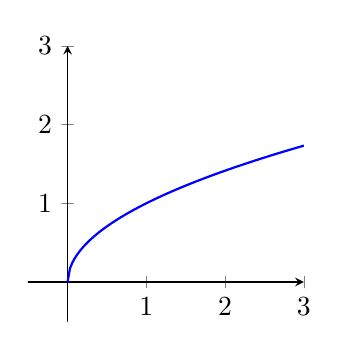
\begin{tikzpicture}[line cap=round,line join=round,>=triangle 45,x=1.0cm,y=1.0cm]
\begin{axis}[
x=1.0cm,y=1.0cm,
axis lines=middle,
xmin=-0.5,
xmax=3,
ymin=-0.5,
ymax=3,
xtick={},
ytick={}]
\clip(-.5,-.5) rectangle (3,3);
\draw[line width=.8pt,color=qqqqff,samples=100,domain=0:3] plot(\x,{sqrt((\x))});
\end{axis}
\end{tikzpicture}
\end{center}
\end{minipage}
\begin{minipage}{.49\linewidth}
\setlength{\parskip}{.3em}
$g$ est continue à droite en $x_{0} = 0$
\end{minipage}
\end{center}
\end{enumerate}

\paragraph{Définitions:}

\begin{itemize}
\item On dit que $f$ est continue sur $[\ a; b\ ]$ si elle continue sur $]a;b[$,
continue à droite en $x = a$ et à gauche en $x = b$

\item Soit $f$ définie sur voisinage pointé de $x_{0}$ avec $x_{0} \notin
\mathbb{D}_{f}$. On dit que $f$ est prolongeable par continuité en $x_{0}$
si $$\lim_{x \to x_{0}} f(x) \text{ existe } (\text{vaut } a \in \mathbb{R})$$

\begin{center}
\begin{minipage}{.5\linewidth}
\begin{center}
\begin{tikzpicture}[line cap=round,line join=round,>=triangle 45,x=1.0cm,y=1.0cm]
\begin{axis}[
x=1.0cm,y=1.0cm,
axis lines=middle,
xmin=-0.5,
xmax=4.0,
ymin=-0.5,
ymax=2.5,
xtick={},
ytick={},]
\clip(-0.5,-0.5) rectangle (4.,2.5);
\draw[line width=.8pt,color=qqqqff,samples=100,domain=1:3] plot(\x,{sqrt((\x))});
\draw [line width=0.4pt,dash pattern=on 3pt off 3pt,color=qqqqff] (2.037512271204936,1.427414540771158)-- (2.037512271204936,0.) node [anchor=north]{$x_0$};
\draw [line width=0.4pt,dash pattern=on 3pt off 3pt,color=ffqqqq] (2.037512271204936,1.427414540771158)-- (0.,1.427414540771158) node [anchor=east]{$a$};
\begin{scriptsize}
\draw [fill=ffqqqq] (2.037512271204936,1.427414540771158) circle (2.0pt);
\end{scriptsize}
\end{axis}
\end{tikzpicture}
\end{center}
\end{minipage}
\begin{minipage}{.49\linewidth}
\setlength{\parskip}{.3em}
On peut alors définie $\tilde f (x)$ continue en $x_{0}$ en
posant
$$ \tilde f (x) = \left\{
\begin{array}{ll}
f(x) & \text{ si } x \neq x_{0}\\
a& \text{ si } x = x_{0}\\
\end{array}
\right.$$
$\tilde f(x)$ est appelé la \textbf{prolongée par continuité}
de $f$ en $x_{0}$.
\end{minipage}
\end{center}

\paragraph{Exemple:}
$$f(x) = \frac{\sin(x)}{x}, \quad x_{0} = 0$$
\begin{center}
\begin{minipage}{.5\linewidth}
\begin{center}
\begin{tikzpicture}[line cap=round,line join=round,>=triangle 45,x=1.0cm,y=1.0cm]
\begin{axis}[
%x=1.0cm,y=1.0cm,
width=\linewidth,
height=4.5cm,
axis lines=middle,
xmin=-15.0,
xmax=15.0,
ymin=-0.5,
ymax=1.5,
xtick={},
ytick={},]
\clip(-15.,-0.5) rectangle (15.,1.5);
\draw[line width=0.4pt,color=qqqqff,smooth,samples=100,domain=-15.0:15.0] plot(\x,{sin(((\x))*180/pi)/(\x)});
\begin{scriptsize}
\draw [fill=ffqqqq] (0.,1.) circle (2.0pt);
\end{scriptsize}
\end{axis}
\end{tikzpicture}
\end{center}
\end{minipage}
\begin{minipage}{.49\linewidth}
\setlength{\parskip}{.3em}
$$\lim_{x \to 0} f(x) = 1$$

$ \tilde f (x) = \left\{
\begin{array}{ll}
\frac{\sin(x)}{x} & \text{ si } x \neq 0\\
1& \text{ si } x = 0\\
\end{array}
\right.$ est $\mathbb{C}^{0}_{\mathbb{R}}$
\end{minipage}
\end{center}
\end{itemize}

\paragraph{Théorème de la valeur intermédiare}
\label{par:theoreme_de_la_valeur_intermediare}

Soit $f$ continue sur $[\ a; b\ ]$, si $$f(a)\cdot f(b) < 0$$ 
alors $$\exists x_{0} \in [\ a; b\ ] \tq f(x_{0}) = 0$$

Illustration du cas $f(a) < 0, f(b) > 0$

\begin{center}
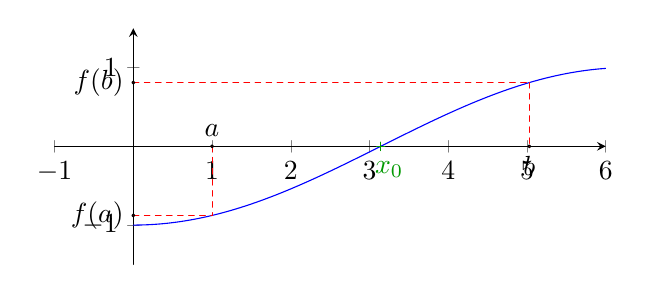
\begin{tikzpicture}[line cap=round,line join=round,>=triangle 45,x=1.0cm,y=1.0cm]
\begin{axis}[
x=1.0cm,y=1.0cm,
axis lines=middle,
xmin=-1.0,
xmax=6.0,
ymin=-1.5,
ymax=1.5,
xtick={},
ytick={},]
\clip(-1.,-1.5) rectangle (6.,1.5);
\draw[line width=0.4pt,color=qqqqff,smooth,samples=100,domain=0:6.0] plot(\x,{0-cos((1.0/2.0*(\x))*180/pi)});
\draw [line width=0.4pt,dash pattern=on 2pt off 2pt,color=ffqqqq] (0.,-0.8775825618903728)-- (1.,-0.8775825618903728);
\draw [line width=0.4pt,dash pattern=on 2pt off 2pt,color=ffqqqq] (0.,0.8097689653851586)-- (5.029109162112794,0.8097689653851586);
\draw [line width=0.4pt,dash pattern=on 2pt off 2pt,color=ffqqqq] (5.029109162112794,0.8097689653851586)-- (5.029109162112794,0.);
\draw [line width=0.4pt,dash pattern=on 2pt off 2pt,color=ffqqqq] (1.,0.)-- (1.,-0.8775825618903728);
\begin{scriptsize}
\draw [color=qqzzqq] (3.141592653589793,0.)-- ++(-1.5pt,0 pt) -- ++(3.0pt,0 pt) ++(-1.5pt,-1.5pt) -- ++(0 pt,3.0pt);
\draw[color=qqzzqq] (3.248747444593085,-0.2913852161132486) node {$x_0$};
\draw [fill=ffqqqq] (1.,0.) circle (0.5pt) node [anchor=south] {$a$};
\draw [fill=ffqqqq] (5.029109162112794,0.) circle (0.5pt) node [anchor=north] {$b$};
\draw [fill=ffqqqq] (0.,-0.8775825618903728) circle (0.5pt) node [anchor=east] {$f(a)$};
\draw [fill=ffqqqq] (0.,0.8097689653851586) circle (0.5pt) node [anchor=east] {$f(b)$};
\end{scriptsize}
\end{axis}
\end{tikzpicture}
\end{center}


\paragraph{Démonstration:}
\label{par:demonstration_}
algorithm de la bisection.

On coupe l'intervalle $[\ a; b\ ]$ en $x = \frac{a+b}{2}$

\begin{itemize}
\item $f\left(\frac{a+b}{2}\right) = 0, \quad x_{0} = \frac{a+b}{2}$
\item $f\left(\frac{a+b}{2}\right) < 0$, alors on pose $$I_{1} = [\ a_{1};
b_{1}\ ] \text{ avec } a_{1} = \frac{a+b}{2} \text{ et } b_{1} = b$$
\item $f\left(\frac{a+b}{2}\right) > 0$, alors on pose $$I_{1} = [\ a_{1};
b_{1}\ ] \text{ avec } b_{1} = \frac{a+b}{2} \text{ et } a_{1} = a$$
\end{itemize}

On réitère le découpage sur l'intervalle $I_{1} = [\ a_{1}; b_{1}\ ]$ et ainsi
de suite :

\begin{itemize}
\item Soit $n \in \mathbb{N}^{*} \tq f \left(\frac{a_{n} + b_{n}}{2}\right)
\text{ et alors } \frac{a_{n} + b_{n}}{2}$

\item Soit on obtient $(a_{n})$ et $(b_{n}), n \in \mathbb{N}^{*}$, 2
suites telles que
        
\begin{itemize}
\item $f(a_{n}) < 0 < f(b_{n})$
\item $b_{n} - a_{n} = \frac{b - a }{2^{n}}$
\item $a \leq a_{1} \leq a_{2} \leq ... \leq a_{n} \leq b_{n} \leq
b_{n-1} \leq ... \leq b_{1} \leq b$
\end{itemize}

$(a_{n})$ est croissante et majorée

$(b_{n})$ est décroissante et minorée

Donc ces suites sont convergentes

Or $$ \lim_{n \to \infty} (a_{n} - b_{n}) = \lim_{n \to \infty} \left(\frac{a-b}{2^{n}}\right)
= 0$$
Donc $$ \lim_{n \to \infty} (a_{n}) = \lim_{n \to \infty} (b_{n}) \text{ (car
les deux limites existent) }$$
Posons $$x_{0} = \lim_{n \to \infty} (a_{n}) = \lim_{n \to \infty} (b_{n})$$
Or $f$ est continue sur $[\ a; b\ ]$ alors $$ \lim_{n \to \infty} f(a_{n})
= \lim_{n \to \infty} f(b_{n}) = f(x_{0})$$
Mais $$f(a_{n}) < 0 < f(b_{n})$$
Donc $$f(a_{n}) = f(b_{n}) = 0$$
D'où $$f(x_{0}) = 0$$
\cqfd
\end{itemize}

\paragraph{Corollaire:}

Soit $f$ continue sur $[\ a; b\ ]$ 

Si $c$ est compris entre $f(a)$ et $f(b)$, alors $$\exists x_{0} \in [\ a; b\ ]
\tq f(x_{0}) = c$$

\begin{center}
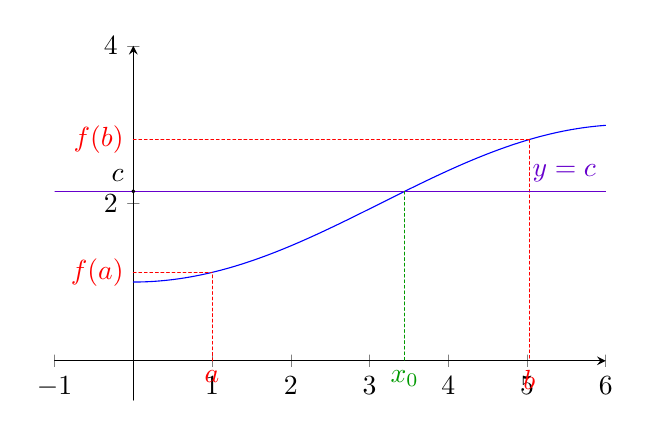
\begin{tikzpicture}[line cap=round,line join=round,>=triangle 45,x=1.0cm,y=1.0cm]
\begin{axis}[
x=1.0cm,y=1.0cm,
axis lines=middle,
xmin=-1.0,
xmax=6.0,
ymin=-0.5,
ymax=4.0,
xtick={},
ytick={},]
\clip(-1.,-0.5) rectangle (6.,4.);
\draw[line width=0.4pt,color=qqqqff,smooth,samples=100,domain=0:6.0] plot(\x,{0-cos((1.0/2.0*(\x))*180/pi)+2.0});
\draw [line width=0.4pt,dash pattern=on 1pt off 1pt,color=ffqqqq] (0.,1.1224174381096272) node [anchor = east]{$f(a)$}-- (1.,1.1224174381096272);
\draw [line width=0.4pt,dash pattern=on 1pt off 1pt,color=ffqqqq] (0.,2.8097689653851585)node [anchor = east]{$f(b)$}-- (5.029109162112794,2.8097689653851585);
\draw [line width=0.4pt,dash pattern=on 1pt off 1pt,color=ffqqqq] (5.029109162112794,2.8097689653851585)-- (5.029109162112794,0.) node [anchor = north]{$b$};
\draw [line width=0.4pt,dash pattern=on 1pt off 1pt,color=ffqqqq] (1.,0.) node [anchor = north]{$a$}-- (1.,1.1224174381096272);
\draw [line width=0.4pt,color=wwqqcc,domain=-1.:6.] plot(\x,{(-2.152086494778833-0.*\x)/-1.}) node [anchor=south east]{$y=c$};
\draw [line width=0.4pt,dash pattern=on 1pt off 1pt,color=qqzzqq] (3.4469506212485506,2.152086494778833)-- (3.4469506212485506,0.) node [anchor = north]{$x_0$};
\begin{scriptsize}
\draw [fill=wwqqcc] (0.,2.152086494778833) circle (0.5pt) node [anchor=south east]{$c$};
\end{scriptsize}
\end{axis}
\end{tikzpicture}
\end{center}

\paragraph{Théorème:}

Soit $f$ continue sur $[\ a; b\ ]$
\begin{itemize}
\item Si $f$ est strictement croissante sur $[\ a; b\ ]$ alors $f$ est
bijective de $[\ a; b\ ]$ sur $[\ f(a); f(b)\ ]$
\item Si $f$ est strictement décroissante sur $[\ a; b\ ]$ alors $f$ est
bijective de $[\ a; b\ ]$ sur $[\ f(b); f(a)\ ]$
\end{itemize}

\paragraph{Démonstration:}

Soit $f$ strictement croissante.

Le théorème de la valeur intermédiaire nous donne l'existence d'un antécédent
pour out $y \in [\ f(a); f(b)\ ]$ et cet antécédent est \textbf{unique} car $f$ est
strictement monotone.

\cqfd

\end{document}
